\chapter{Implementation}
\label{ch:implementation}

[Brief introduction of the chapter]

Being a blockchain project, the goal is to not use the so called Web2 technologies, this means the traditional approaches of having a backend running on a server and similar services, but rather to use only Web3 technologies for us to understand exactly the limitations there are by adopting solely the blockchain ecosystem. Ideally, of course, in the future this project benefits greatly by merging these two approaches.

\section{Solidity}
\label{sec:solidity}

We'll be doing the smart contracts in Solidity, because it's the most popular language for Ethereum smart contracts, and makes it easy to deploy to any EVM compatible blockchain. This language is similar to other languages like C++, but it has some unique features that make it very powerful for smart contracts.

One important aspect is that when a contract is public, anyone can call its functions, that's why we need to restrict their access and take into account that possibility when defining the operations of the entire contract. So it's always important to have a mindset that any function (endpoint) can be called by anyone, which is a pretty different approach from traditional web development.

Another thing is that contracts run atomically, so if something should fail or revert, the changes don't take place. Modifiers are a good example where it can be used to prevent reentrancy attacks, which are a common security issue in smart contracts, and restrict the access to certain functions, reverting if an intruder tries to call them.

We can define, for example, a call to register an event to be restricted to only organizers or a call to validate tickets to be limited to only validators. This is possible because there are a few keywords like \textit{msg.sender} that tell us which user address called the function and \textit{msg.value} that tell us how much value was sent with the transaction. This value is essentially the amount of money the user sends in a transaction, necessary, for example, to buy the tickets. We'll check if the value matches the correct price and reverts otherwise.

Each blockchain network has its own currency, in which is commonly referred to as ether, on the EVM networks. This is the unit of value that is used to pay to execute transactions, but in solidity we cannot work with floating point numbers, so we have to work with the smallest unit of ether, which is called wei. Similar to how we have 1 euro is 100 cents, we have 1 ether is $10^{18}$ wei, same as on the bitcoin network we have the 1 bitcoin (BTC) is $10^{8}$ satoshis (SATS). This is the unit being used when we call the \textit{msg.value} variable, so we always have to account for the conversion.

Another unique feature of Solidity is the \textit{address} type, which is basically a string strict to the Ethereum address format. That's how we'll be storing the addresses of the organizers and the events on the contracts. The only difference between a user and a contract is that a contract has code associated with it, so it can execute functions and store data, while a user can only send transactions.

This way we can understand why, to send a transaction, paying for the tickets for example, we send value along with it, matching the expected price according the logic of the buy method. Essentially we're sending money to the contract, which is stored in the contract's balance, like a normal user wallet. This is how the contract can store money and manage it, for then the organizer to withdraw its profit to his own wallet.

The deployment will be done using \href{https://book.getfoundry.sh/}{Foundry}, a toolkit for the development and deployment of the smart contracts, which makes it easy to deploy to any network, and also to test the contracts locally.

\section{Main Smart Contract}
\label{sec:main_smart_contract}

So smart contracts are similar to C++ mainly because it lies on a class-like structure with variables to store data and methods, where the main difference is that a class is called a contract and you can extend others to integrate their functionalities. That's essentially what's gonna happen with each event, extending the ERC721 standard, making it a collection of NFTs, where each NFT is a ticket.

Since this is the behavior we want (each event being a NFT collection), we will have to deploy (instantiate, in C++) a new contract for each event, like the Figure \ref{fig:system_behavior} shows, so we need a main contract to keep track of these events.

\begin{figure}[H]
    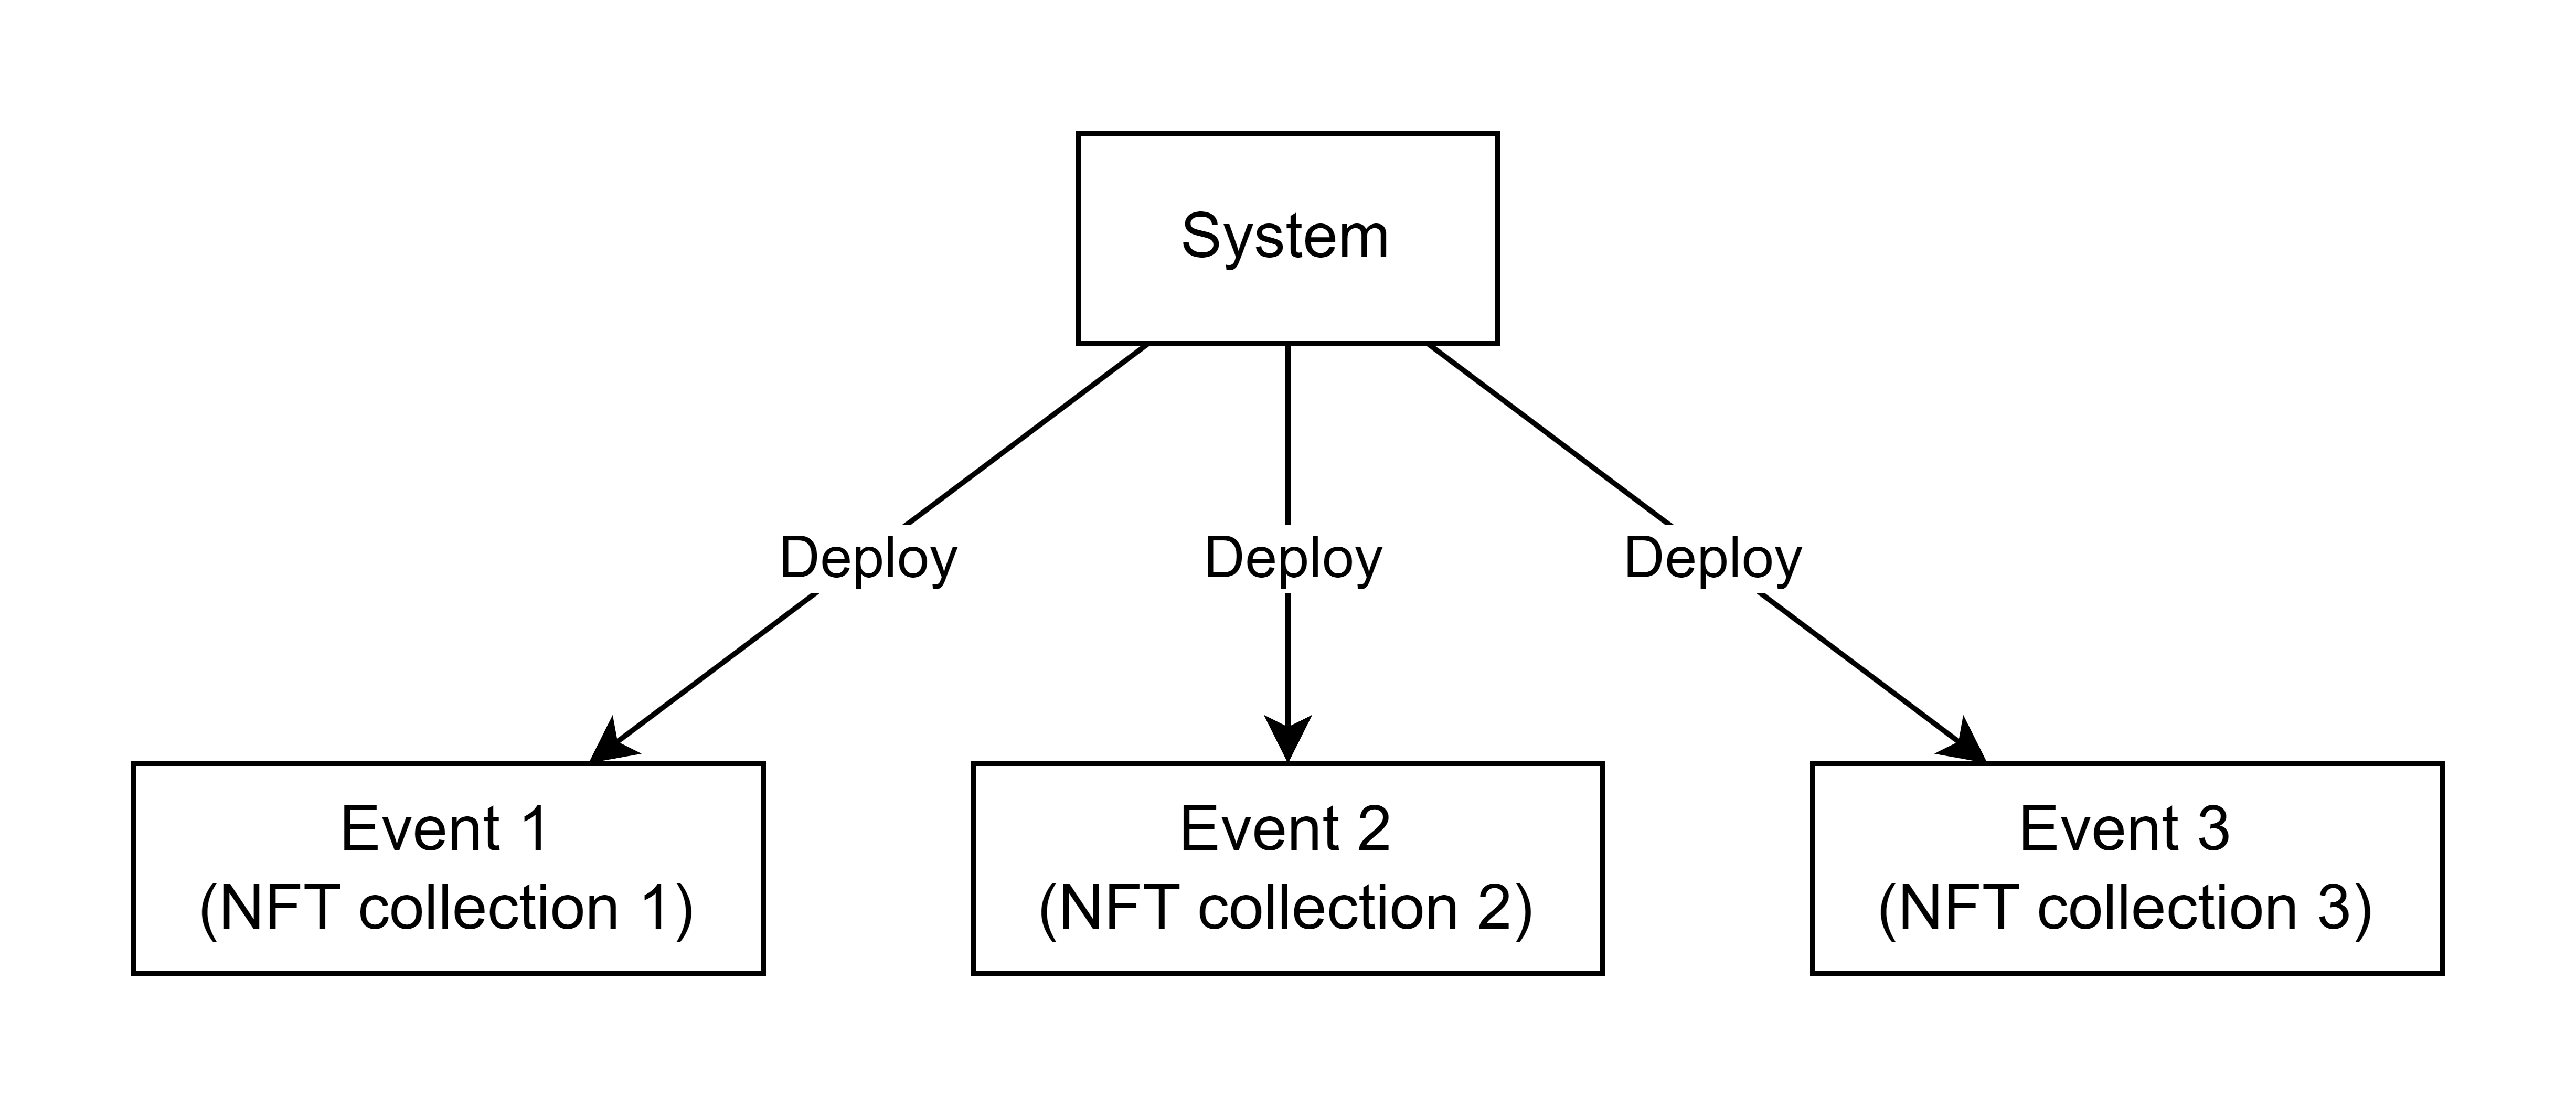
\includegraphics[width=\textwidth*2/3]{System behavior.png}
    \centering
    \caption{System behavior}
    \label{fig:system_behavior}
\end{figure}

With this in mind, like we see in the Figure \ref{fig:system_uml}, the main contract will track the organizers and the events associated with the system, along with the method to register a new event with the necessary data, restricted to only organizers (to avoid unauthorized people to interact).

\begin{figure}[H]
    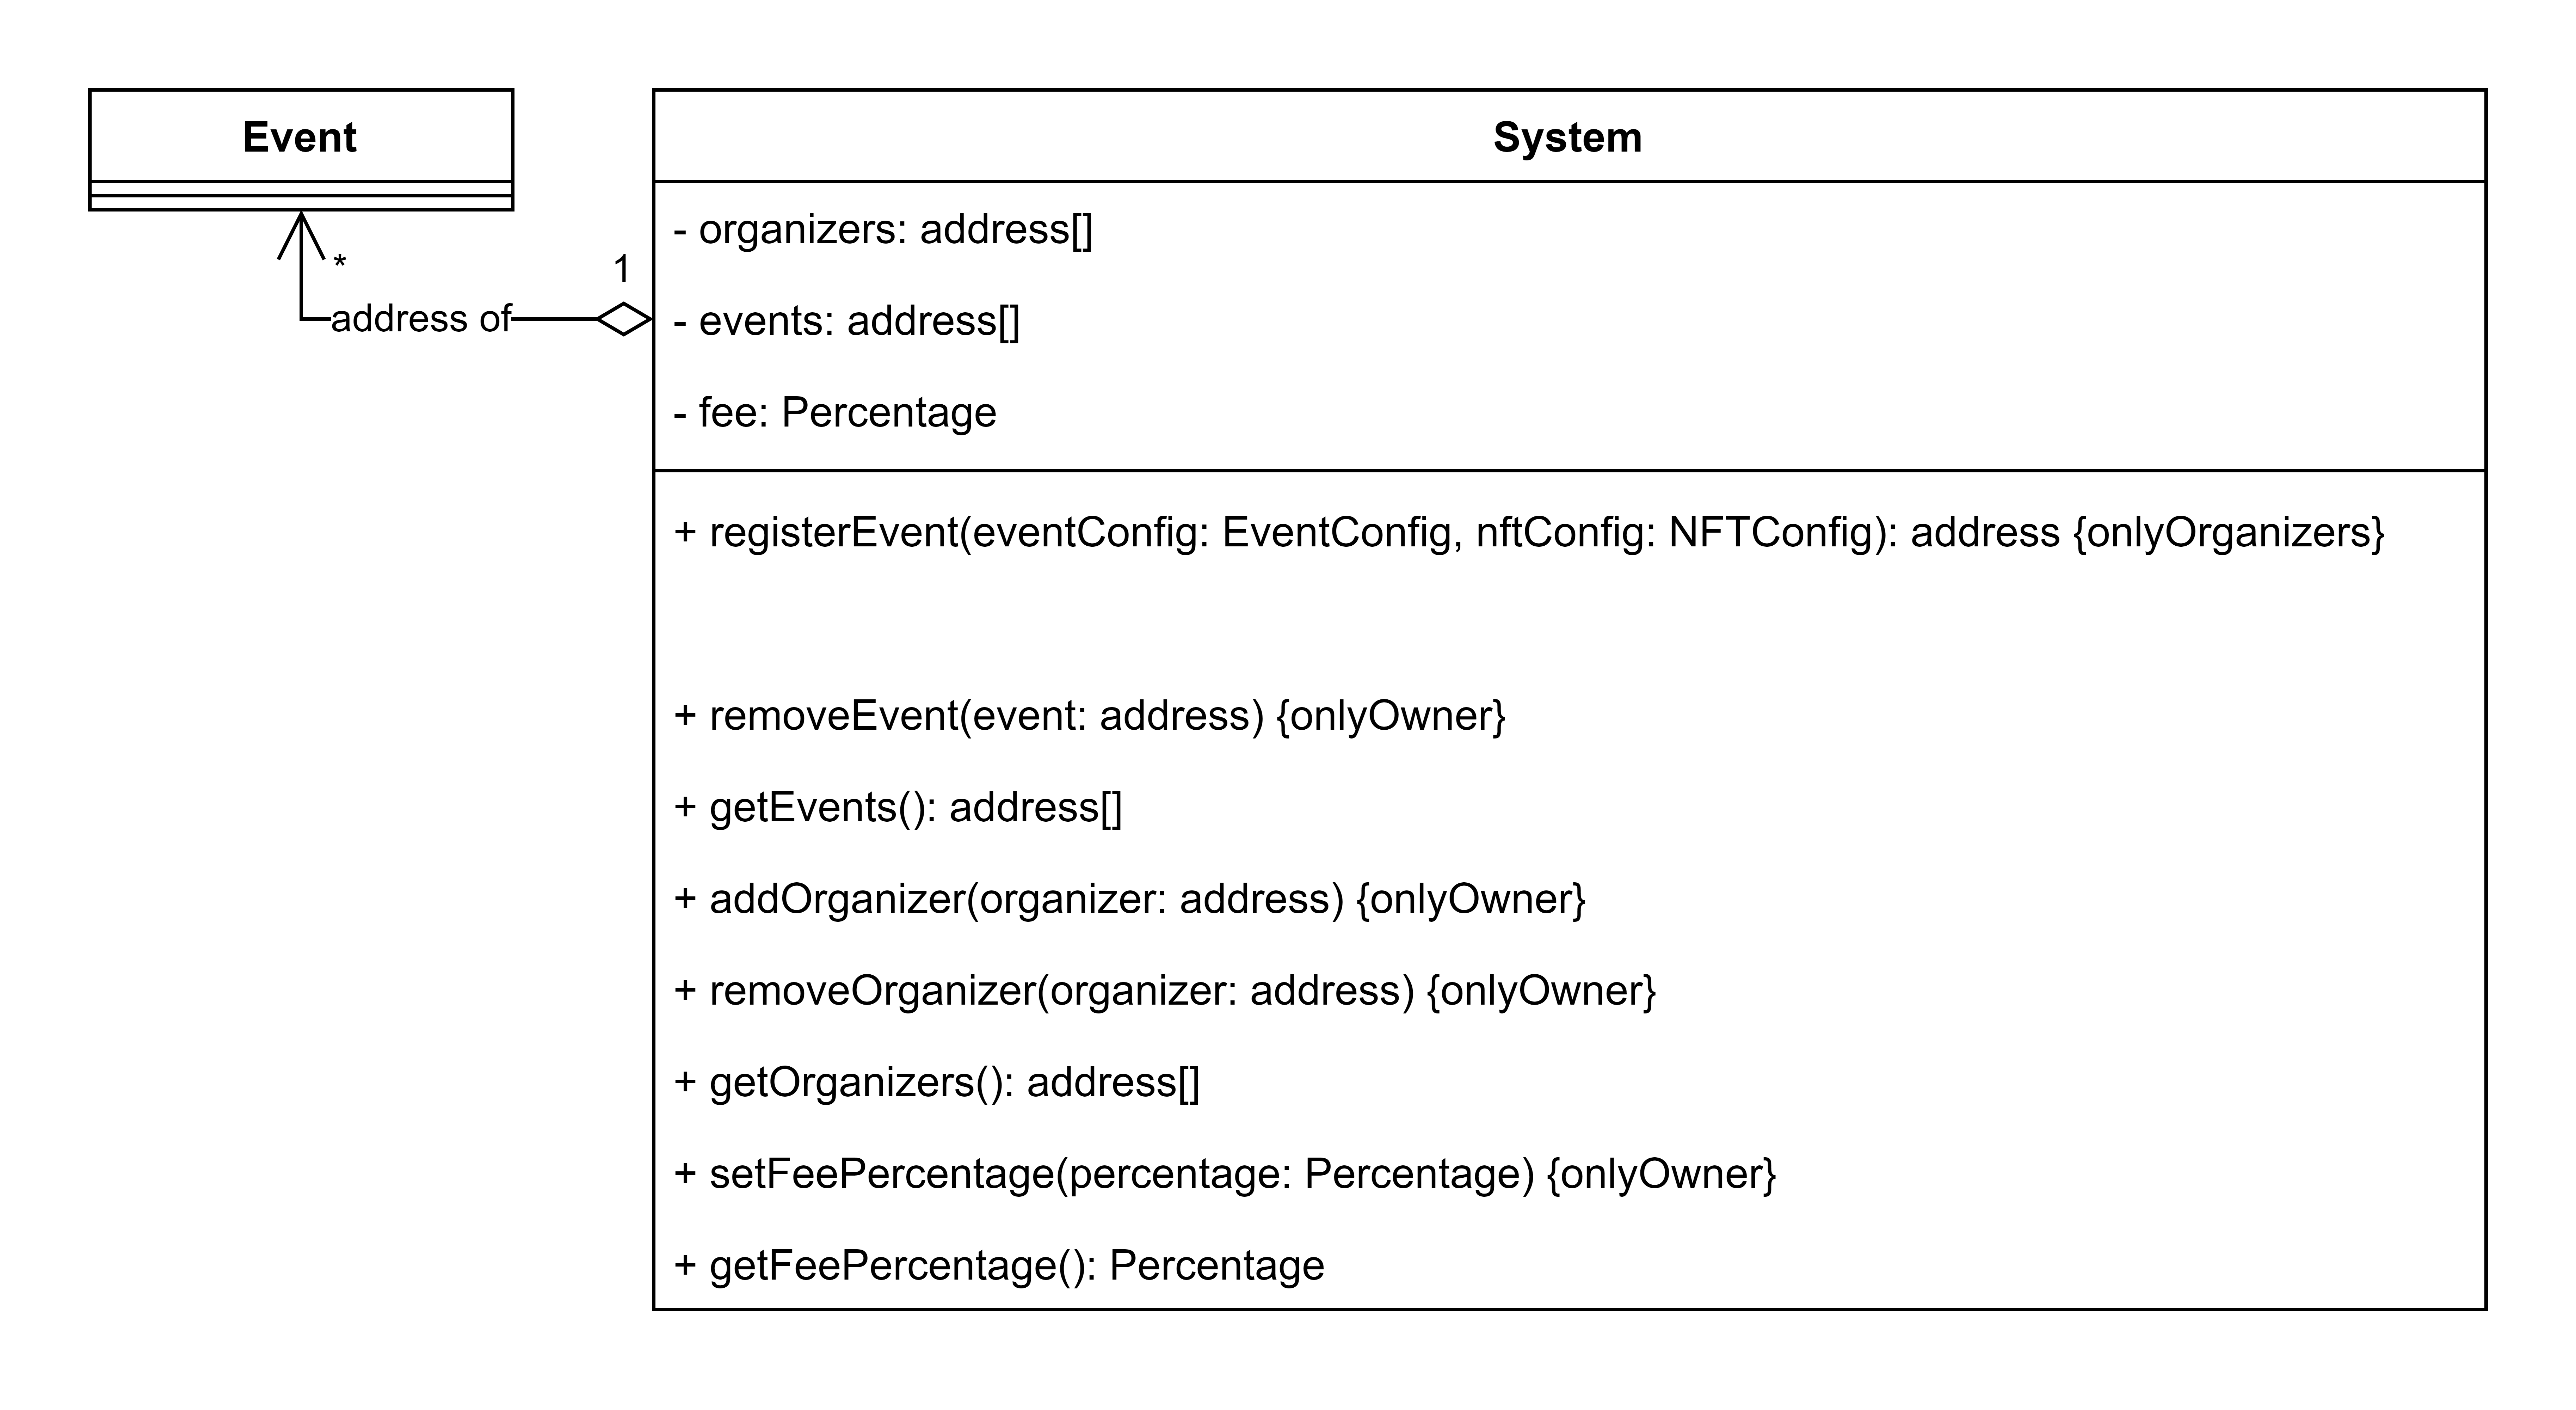
\includegraphics[width=\textwidth]{System UML.png}
    \centering
    \caption{Main smart contract UML}
    \label{fig:system_uml}
\end{figure}

With this structure, since we have this main contract where all the events of the system are stored, we can simply make a call to get them all, showcasing them in the app's home page for users to search. Any event that is deployed outside the system or if it gets removed from there, it won't be shown to the users.

\section{Event Smart Contract}
\label{sec:event_smart_contract}

For the event contract, we'll be extending the ERC721 standard and adding the necessary methods to interact with the tickets, like buying, selling, and validating them. The reason to extend this standard and not implement the logic manually is because it makes it compatible with the most common marketplaces for NFTs, which allows for users to do what they desire with them after the event. It also has the necessary methods to manage the tickets, like transferring them between users, and the necessary operations to track these operations.

\subsection{ERC721 Structure}
\label{subsec:erc721_structure}

The standard was obtained through the \href{https://docs.openzeppelin.com/contracts/api/token/erc721#ERC721}{OpenZeppelin} library, which is a collection of secure and community-vetted smart contracts that are used by many projects in the Ethereum ecosystem. This library is a great resource for developers to build secure and reliable smart contracts.

Analyzing its source code [ref], and looking into the most important variables and methods of the standard shown in the Figure \ref{fig:erc721_uml}, we can understand that the NFTs are simply a mapping of the token ID to the owner address, so when you execute a transaction to get a token (this process is called minting), the token ID is then associated to your address. Then for each token it's possible set a URI, which is a link to the NFTs metadata, usually being a JSON file with the necessary information about the token, like the name, description, and image.

This link could point to anything, for example a google drive file, but the common thing is to store the metadata on the IPFS, which is a decentralized storage system, so the metadata is not stored on the blockchain itself (onchain), which would be very expensive, but rather on a decentralized storage system (offchain), which is much cheaper.

\begin{figure}[H]
    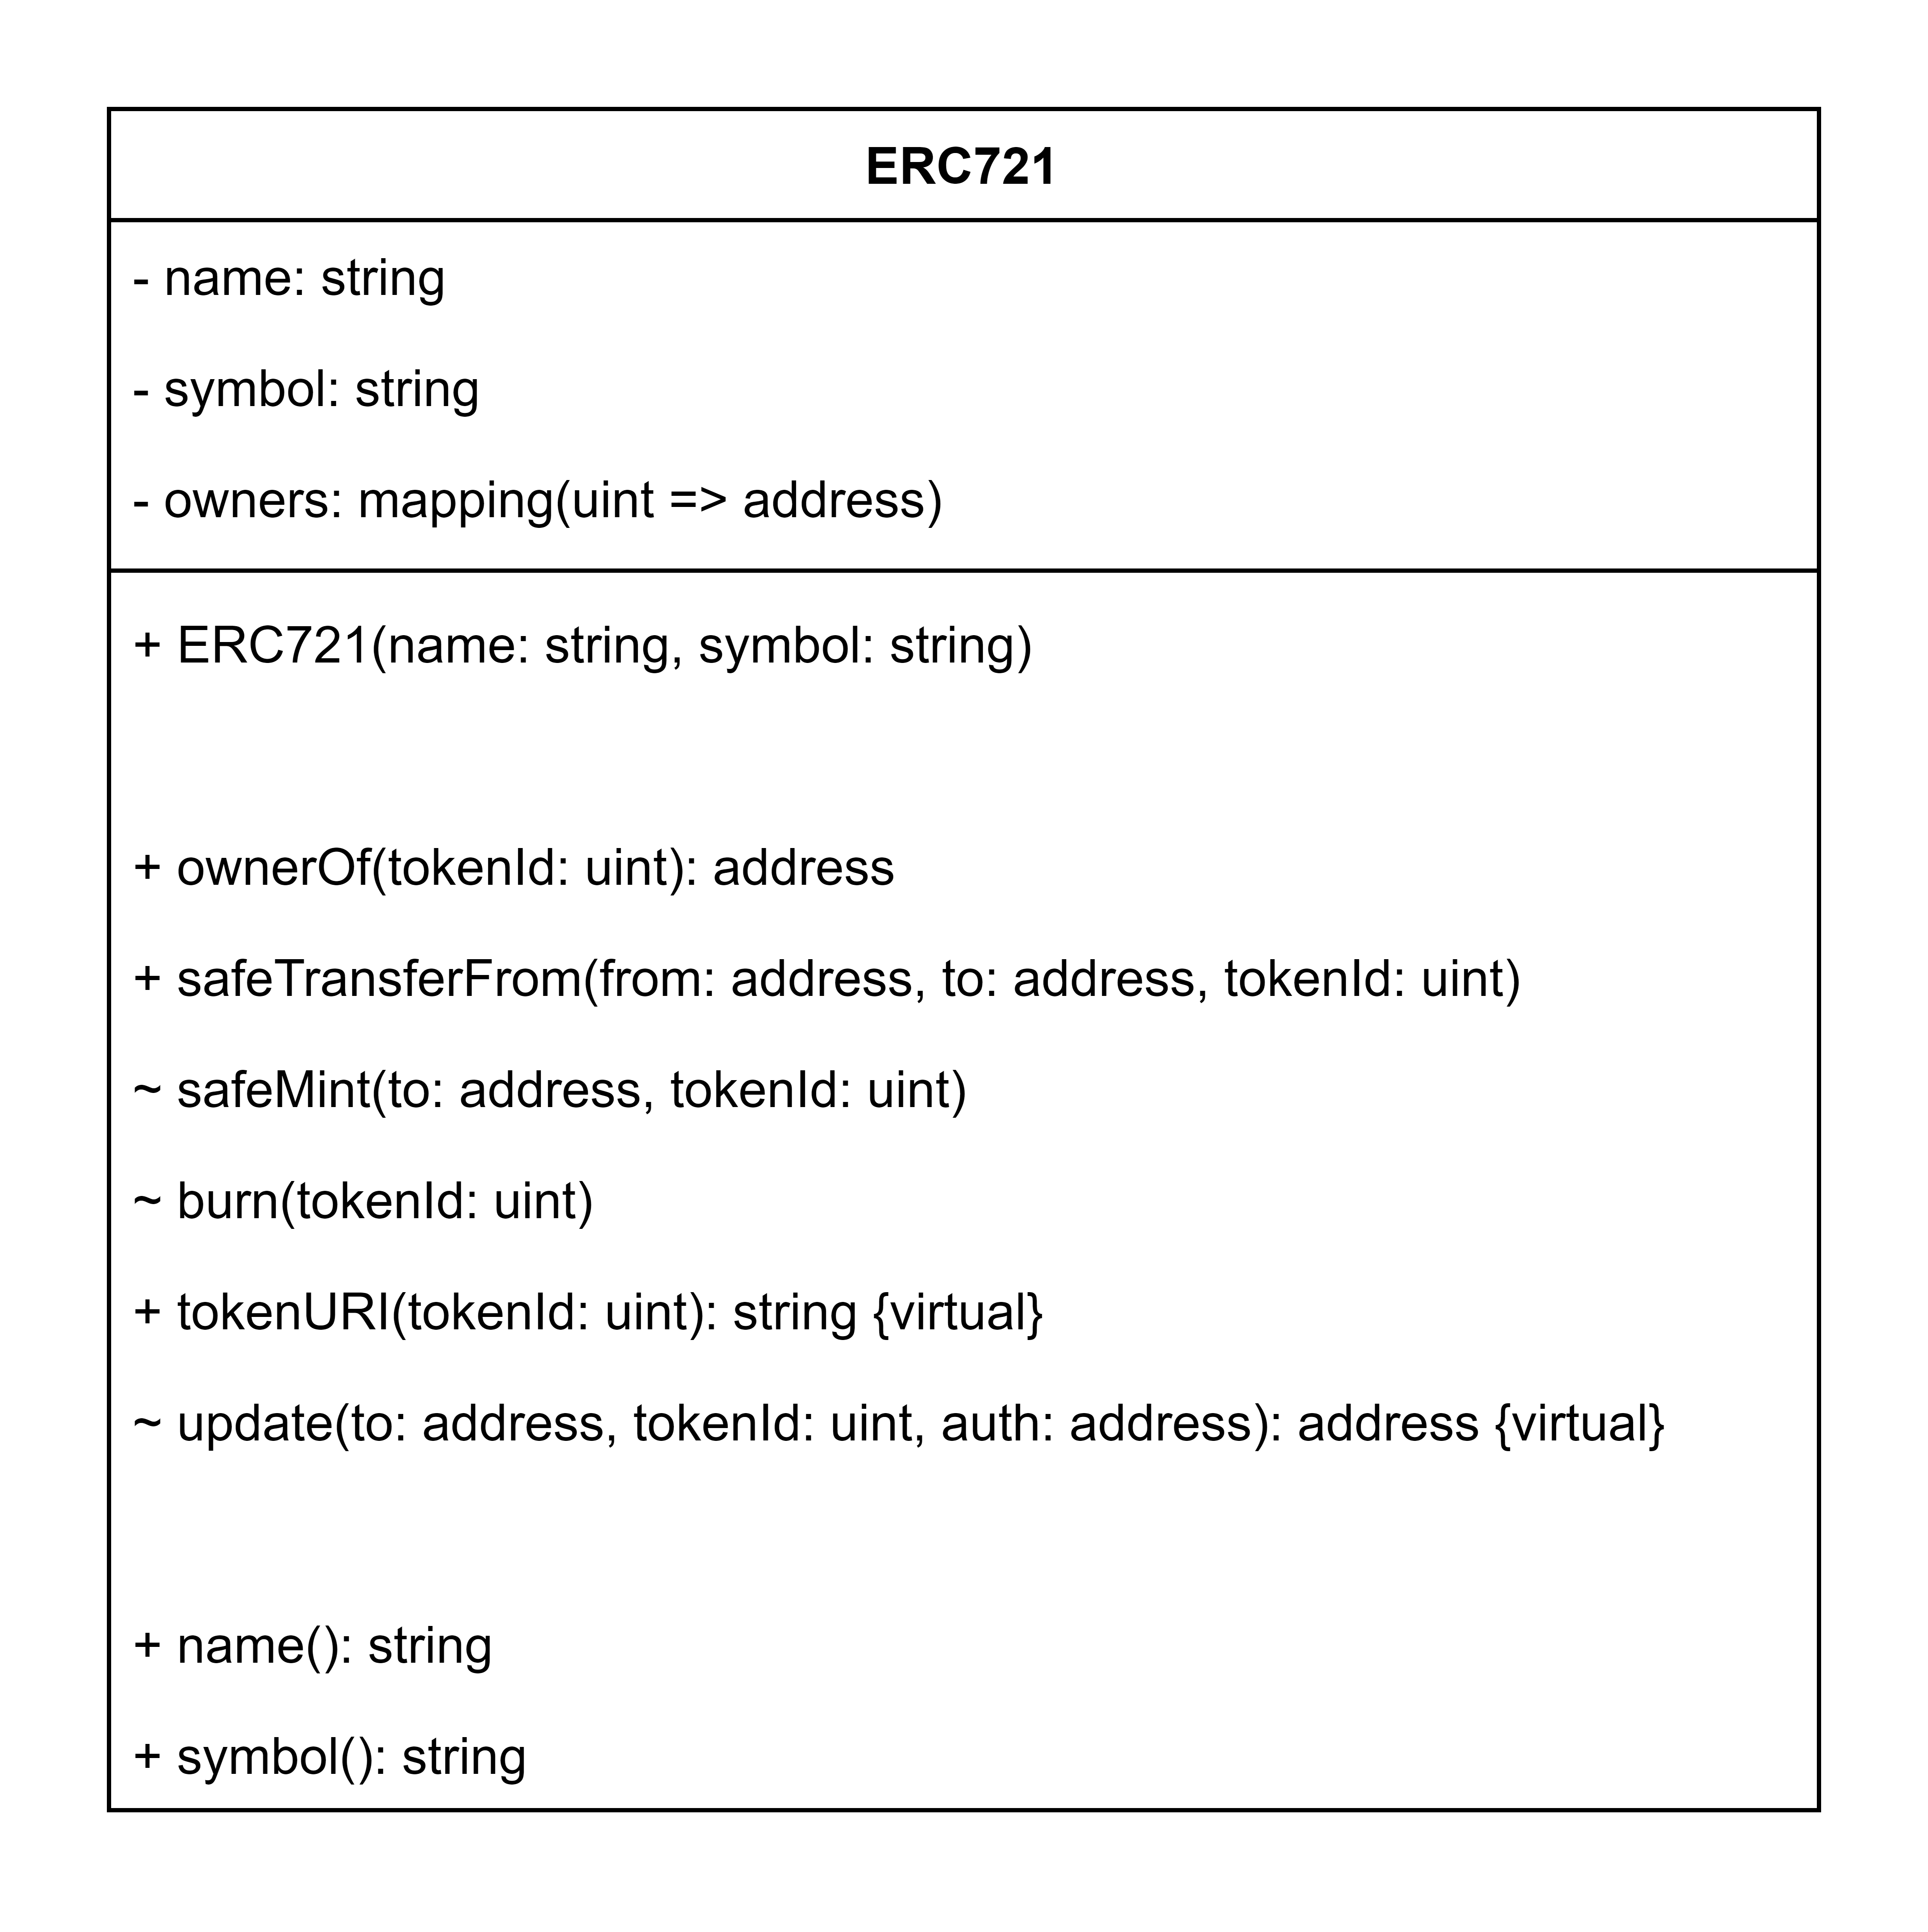
\includegraphics[width=\textwidth*2/3]{ERC721 UML.png}
    \centering
    \caption{ERC721 UML}
    \label{fig:erc721_uml}
\end{figure}

The function \textit{tokenURI} is the one that is called by default in the marketplaces to get the NFT's metadata, being one of the main reasons to extend the ERC721 standard, because it enforces the implementation of this method. In the Figure \ref{fig:erc721_uml} we see that it has the \textit{virtual} keyword, meaning this can be overridden by the contracts that extend it, to manipulate the way to store the metadata. We'll be mentioning this again in the Section \ref{fig:package_logic}, about how the packages logic is implemented.

\subsection{Event Behavior}
\label{subsec:event_behavior}

So the event will be deployed and we need a certain control over the tickets. One of the aspects we need to account for is that when deploying an event, and since the event will extend the ERC721, any public functions on that standard will be possible to execute. This is a problem because we don't want the users to mint tickets whenever they want or transfer them between themselves from outside the system, so we need to restrict these operations. As we saw already on the Figure \ref{fig:erc721_uml}, only the \textit{safeTransferFrom} method is public, so users could transfer NFTs between each other. We want that to be possible, just not from outside the system, since that can lead users to exploit the system and scalping the tickets easily. The minting, however, won't be an issue because it's an internal method, so we will access it from the buy method in the event and restrict it there.

The Figure \ref{fig:event_lifecycle} shows the lifecycle of the event, and what restrictions are in place for the ticket operations. We will have 4 main states for the event after it has been registered, being \textit{Open}, \textit{No refund}, \textit{Start}, and \textit{End} dates. Once the event is registered, it will show up in the app for user to see, and the organizers can set a later open date to allow ticket minting (buying).

\begin{figure}[H]
    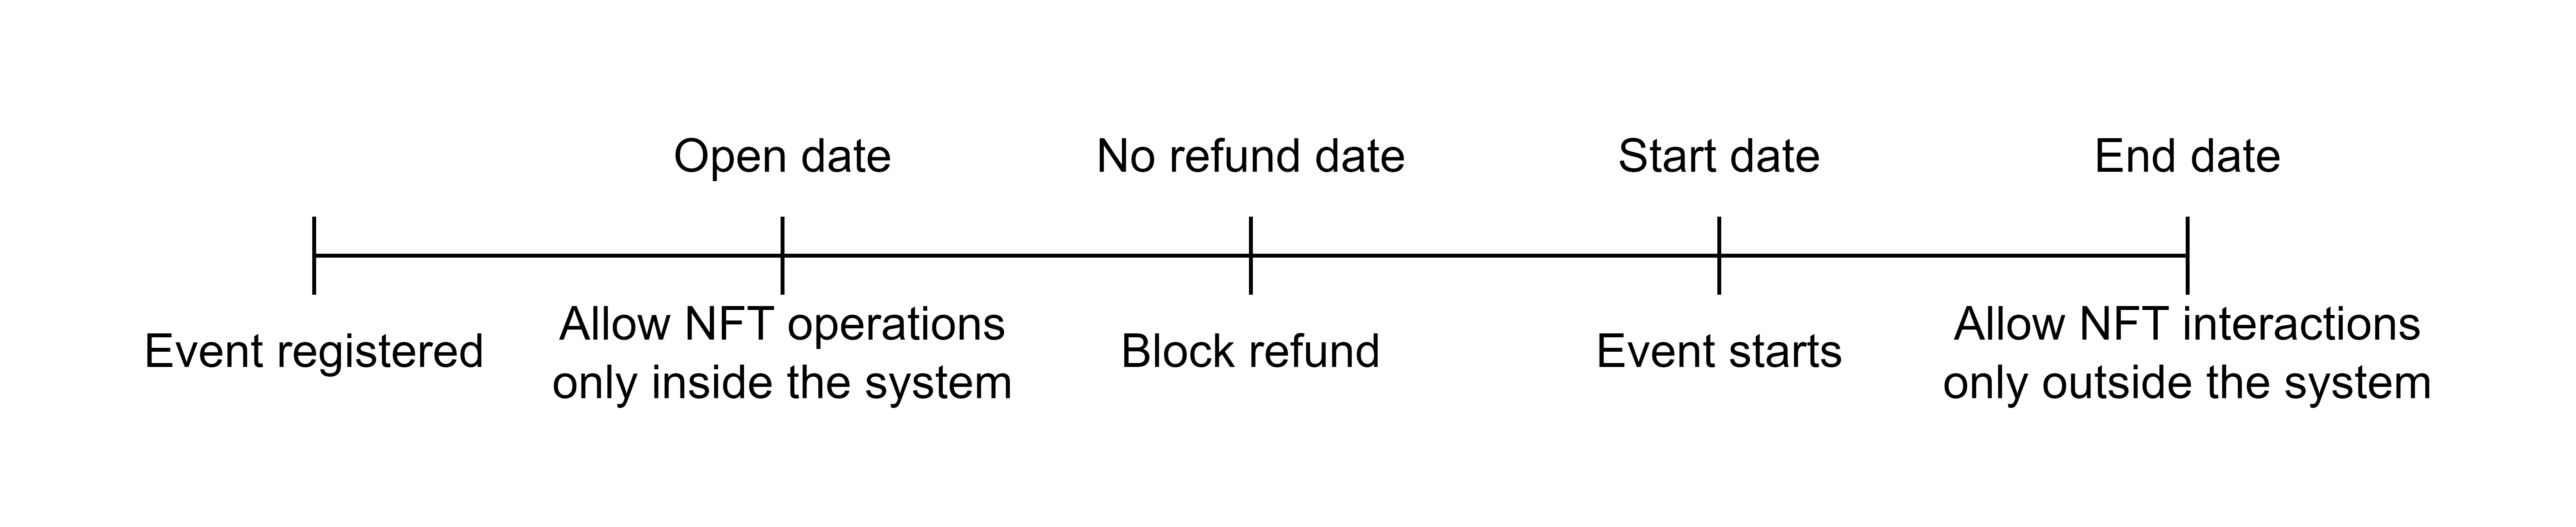
\includegraphics[width=\textwidth]{Event lifecycle.png}
    \centering
    \caption{Event lifecycle}
    \label{fig:event_lifecycle}
\end{figure}

\subsubsection{Open Date}

Once it hits the \textit{Open} date, we will allow the users to buy the tickets, which will mint the NFTs by executing the \textit{safeMint} method of the ERC721 contract.

\subsubsection{No Refund Date}

After the \textit{No refund} date, we will prevent the users to call the refund method, which essentially \textit{burns} the NFTs, removing them from the user and making them available again.
This is a nice operation to add because it allows the users to get their money back if they can't attend the event. The organizer decides the percentage of the refund and the deadline, which is there to prevent users to buy a big amount of tickets and then refund them last minute, which would be a way to exploit the system (in case of a 100\% refund, they wouldn't risk anything).
The other good thing for the organizer is when the event is expected to be sold out. Since the users will get some money back, they will have a reason to refund their tickets if they cannot attend the event anymore, making them available again for other users to buy at the original price, making the organizer a higher profit.
After this deadline, the only that'll be allowed is for users to resell their tickets in the system's marketplace, which them to sell at a higher price than the refund (but never higher than the original, of course).

\subsubsection{Start Date}

The \textit{Start} date is there to tell the users when the event starts, so basically when the gates will open. That's the date that appears in the app, so the users know when to show up.

\subsubsection{End Date}

The \textit{End} date tells when the event is over, unlocking all the ticket operations to outside the system. So users can simply keep the tickets as a souvenir or sell them in any marketplace, without any restrictions on the tickets, including the removal of the price cap.

With this behavior in mind, we came up with the Event UML, like shown in the Figure \ref{fig:event_uml}, where we added the necessary methods for the organizer/admins to manage the event and the users to handle the tickets, which then trigger the corresponding methods of the ERC721 contract. We added a possibility to have admins so the organizer can distribute the workload of executing the necessary operations to people he trusts.

\begin{figure}[H]
    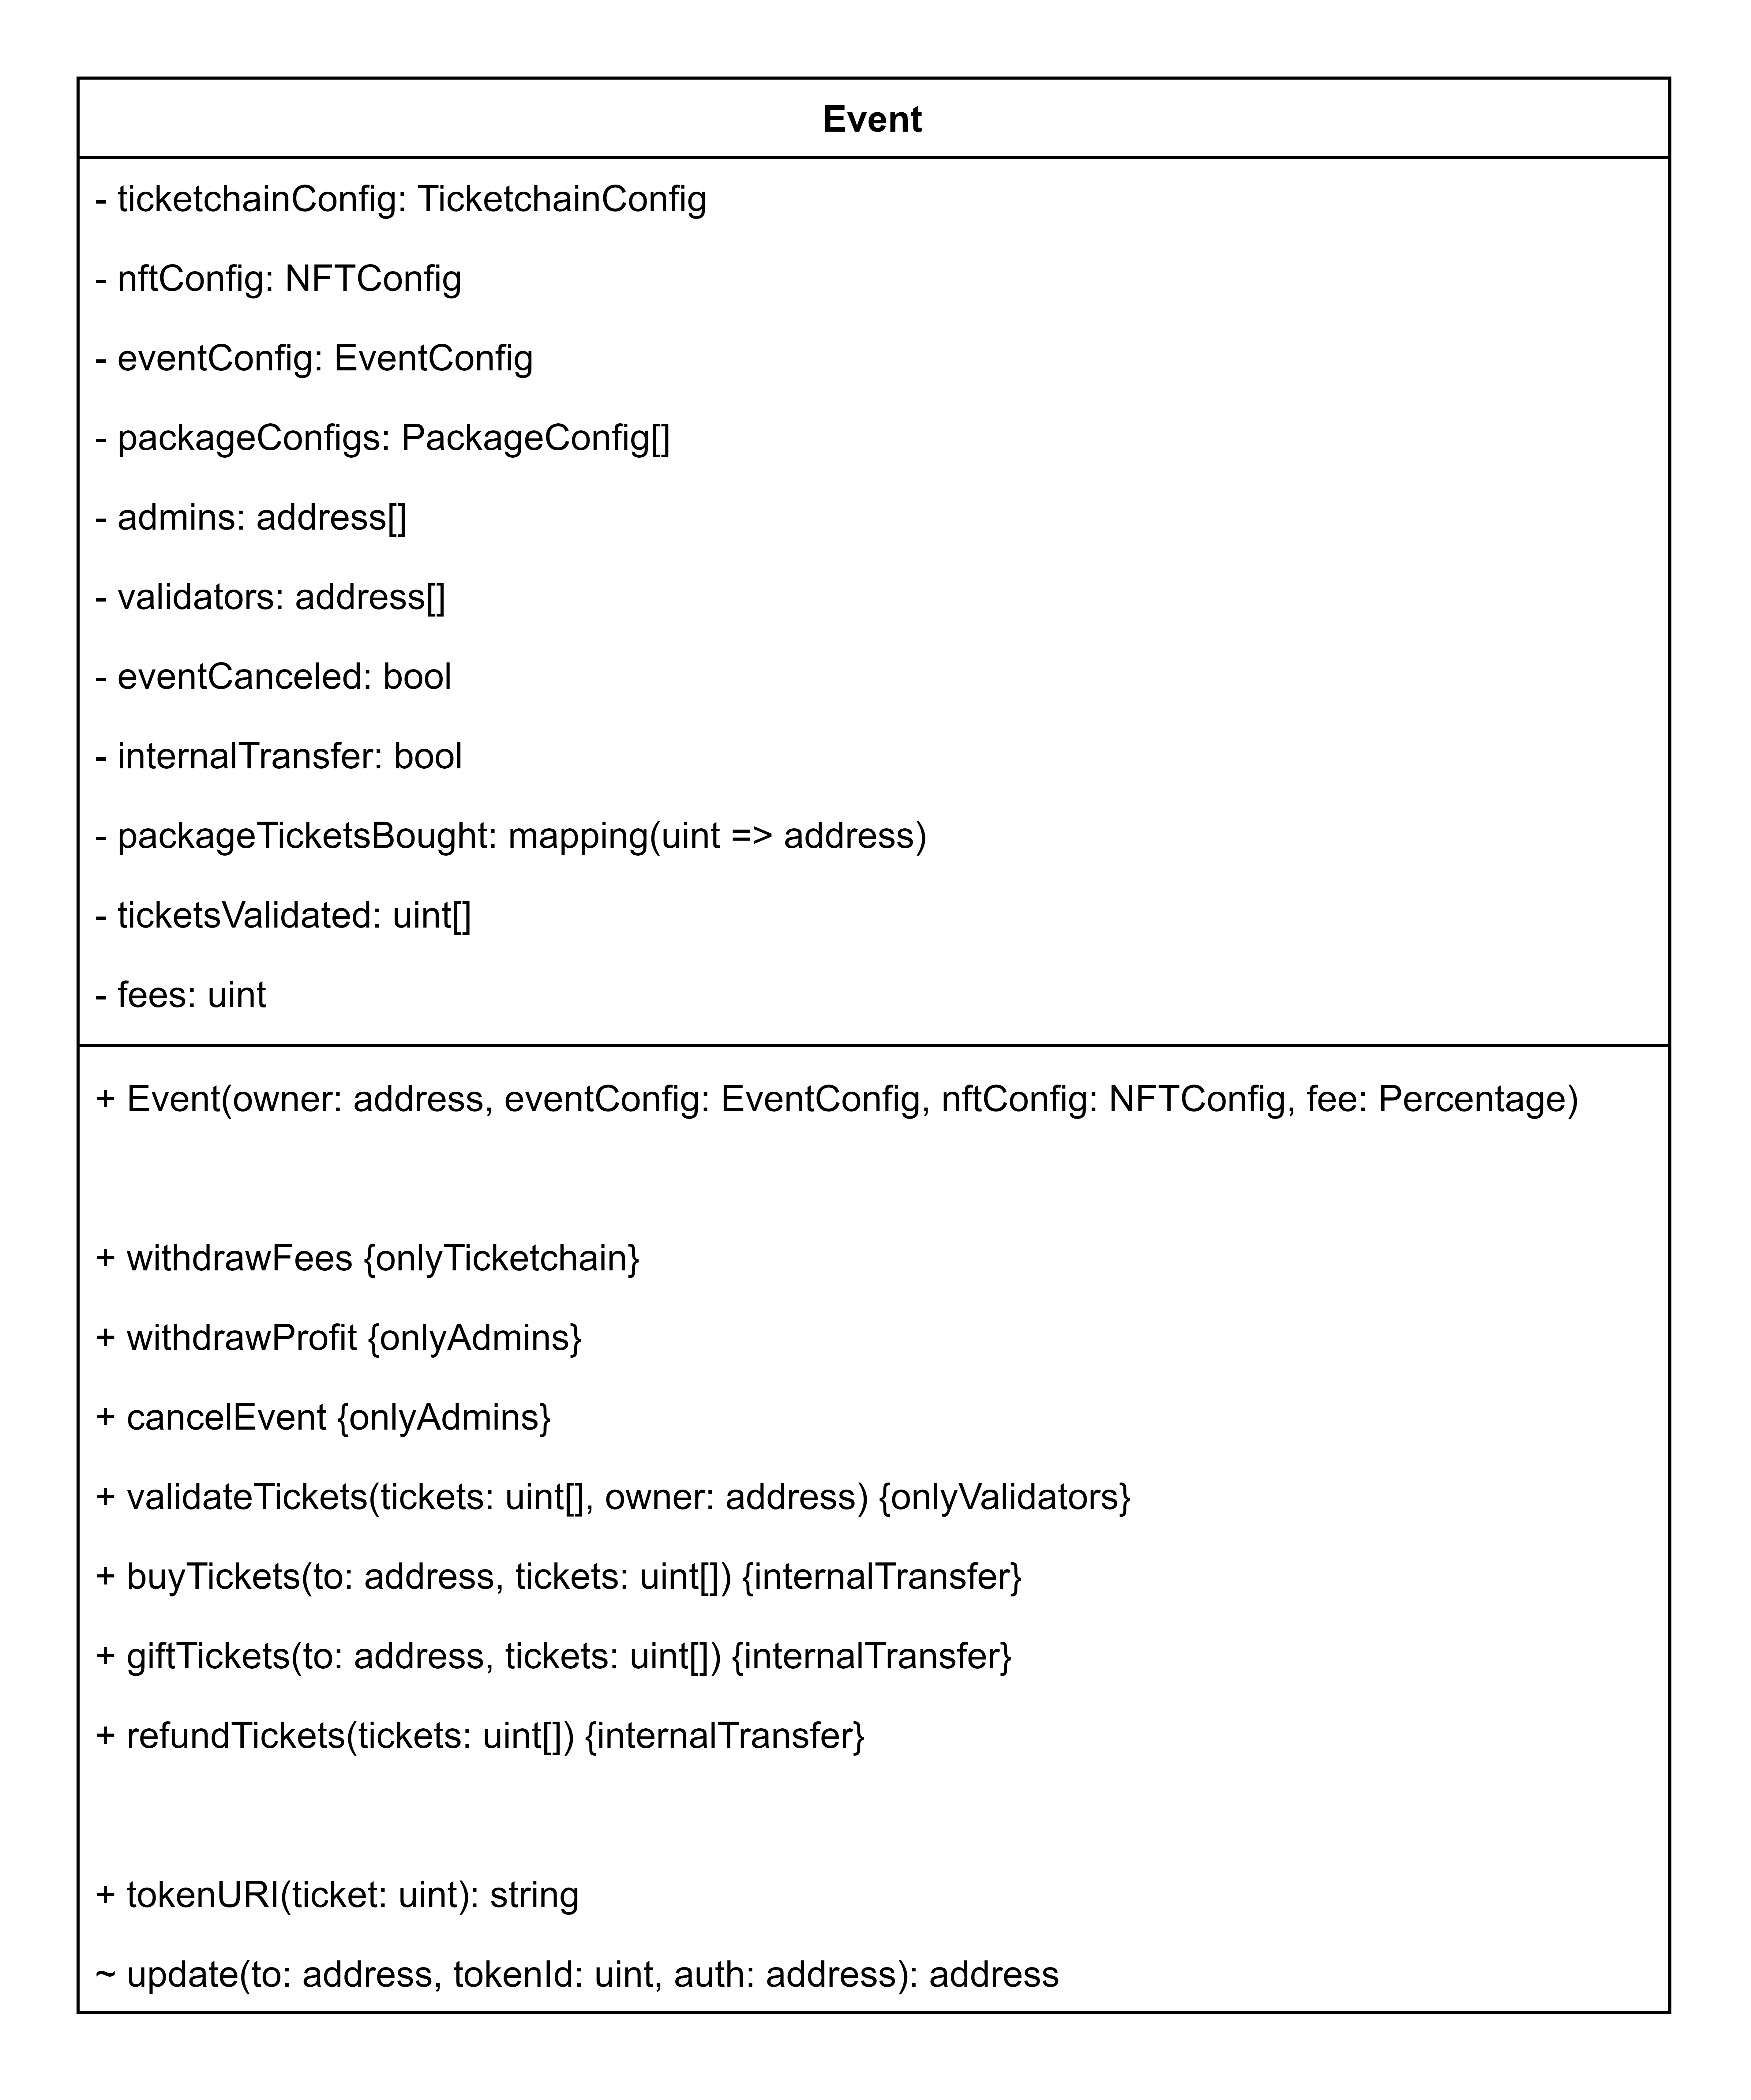
\includegraphics[width=\textwidth*3/4]{Event UML.png}
    \centering
    \caption{Event smart contract UML}
    \label{fig:event_uml}
\end{figure}

As we can see, the \textit{update} method has been overridden from the ERC721 standard, to restrict the interactions with the NFTs according the defined behavior. This method is the one that gets called anytime there's a change in the NFTs state, so we can implement the necessary logic to restrict the operations here and we can visualize it in the following flowchart, shown in the Figure \ref{fig:nft_flowchart}.

\begin{figure}[H]
    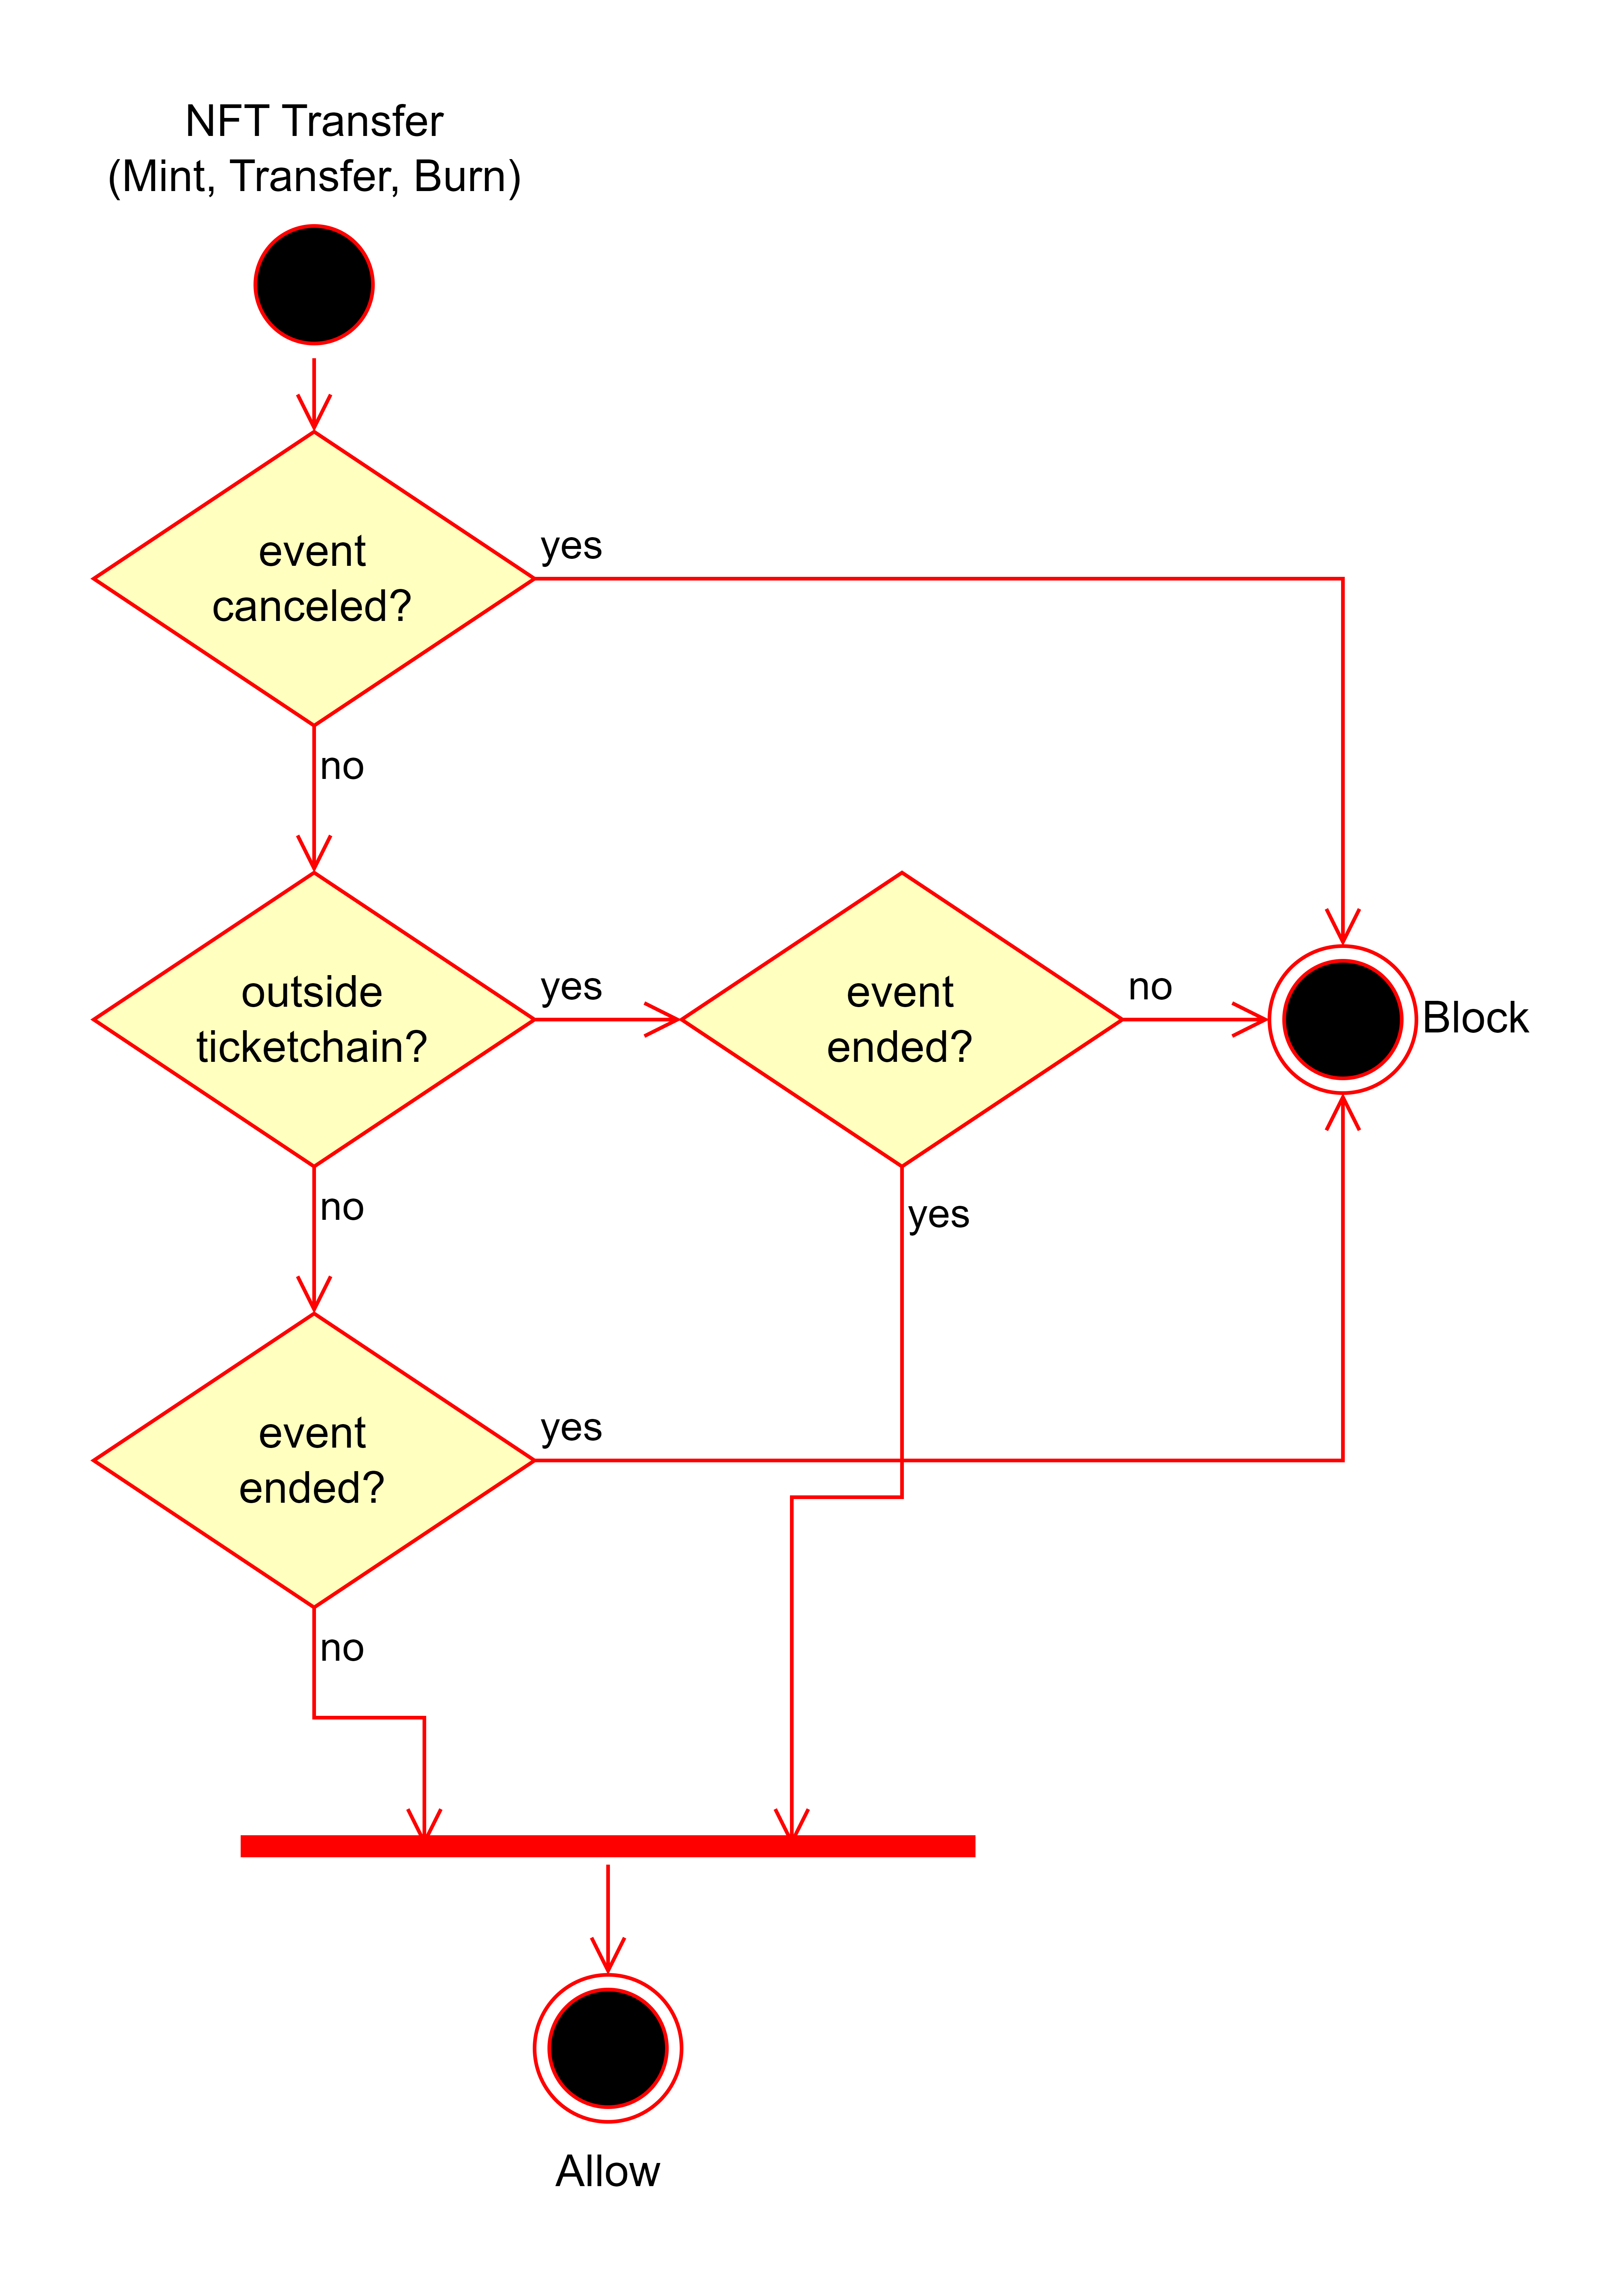
\includegraphics[width=\textwidth*2/3]{NFT flowchart.png}
    \centering
    \caption{NFT flowchart}
    \label{fig:nft_flowchart}
\end{figure}

\subsection{Structs}
\label{subsec:structs}

As is possible to see in the Figure \ref{fig:event_uml}, and also in the Figure \ref{fig:system_uml}, we have a few custom structs to organize better the data. These structs are the \textit{Percentage}, \textit{EventConfig}, \textit{NFTConfig}, \textit{PackageConfig} and \textit{TicketchainConfig} structs.

\subsubsection{Percentage Struct}
\label{subsubsec:percentage_struct}

The \textit{Percentage} struct is necessary because in Solidity there are no floating point numbers, so we need a way to make calculations with percentages. What this struct does is it stores the value of the percentage and the amount of decimals it has, so if we want to calculate 55.50\% of a number, we would have 555 as the value with 1 decimal, or 5550 with 2 decimals.

The struct is as follows:
\begin{verbatim}
    struct Percentage {
        uint256 value;
        uint256 decimals;
    }
\end{verbatim}
so to obtain a percentage of some $x$ number, we do $y = \frac{x \times \text{Percentage.value}}{100\mathrm{e}^\text{Percentage.decimals}}$.

When working with ether units, it can be common to have values like 0.00005 ether, but it's rather rare to have small values in wei, like 1000 wei, so applying this formula won't lose much precision (note that 1 ether is $10^{18}$ wei).

\subsubsection{TicketchainConfig Struct}
\label{subsubsec:ticketchainconfig_struct}

The \textit{TicketchainConfig} struct is simply to keep it stored the system address and the system fee percentage, so we can easily access this information when applying the fees and withdrawing them, and is as follows:
\begin{verbatim}
    struct TicketchainConfig {
        address ticketchainAddress;
        Percentage feePercentage;
    }
\end{verbatim}

\subsubsection{NFTConfig Struct}
\label{subsubsec:nftconfig_struct}

The \textit{NFTConfig} struct is just to store the NFTs basic information, like the name, symbol, and base URI, to ease the input of the NFTs information when registering the event:
\begin{verbatim}
    struct NFTConfig {
        string name;
        string symbol;
        string baseURI;
    }
\end{verbatim}
The is the name of the NFT collection and the symbol is the abbreviation of it, like the name being 'Ticketchain' and the symbol being 'TCK', for example. The base URI is the link to the metadata of the NFTs, which will be used to get the information about the tickets.

\subsubsection{EventConfig Struct}
\label{subsubsec:eventconfig_struct}

The \textit{EventConfig} struct is to store the event's entire configuration, like the name, description, location, dates, and refund, like this:
\begin{verbatim}
    struct EventConfig {
        string name;
        string description;
        string location;
        uint256 openDate;
        uint256 noRefundDate;
        uint256 startDate;
        uint256 endDate;
        Percentage refundPercentage;
    }
\end{verbatim}

\subsubsection{PackageConfig Struct}
\label{subsubsec:packageconfig_struct}

Lastly, the \textit{PackageConfig} struct is there to store each package information, to keep track of the ones that are available for the event:
\begin{verbatim}
    struct PackageConfig {
        string name;
        string description;
        uint256 price;
        uint256 supply;
        bool individualNfts;
    }
\end{verbatim}
This structure will be better discussed in the next Section \ref{subsec:ticket_packages}.

\subsection{Ticket Packages}
\label{subsec:ticket_packages}

It's common to see events with different types of tickets, like VIP, standard, or even 3-day passes, each with its own price and benefits. We want to implement this feature in the system, so we can have a better control over the tickets and the users can choose the one that fits them better.

For that, we will allow the organizer to add packages, indicating the supply of each one, and as we saw already, the NFTs are a mapping of the ID to the owner, so we can organize the packages as a list, where the supply and order of the package defines the ID of each NFT, like the Figure \ref{fig:package_logic} demonstrates.

\begin{figure}[H]
    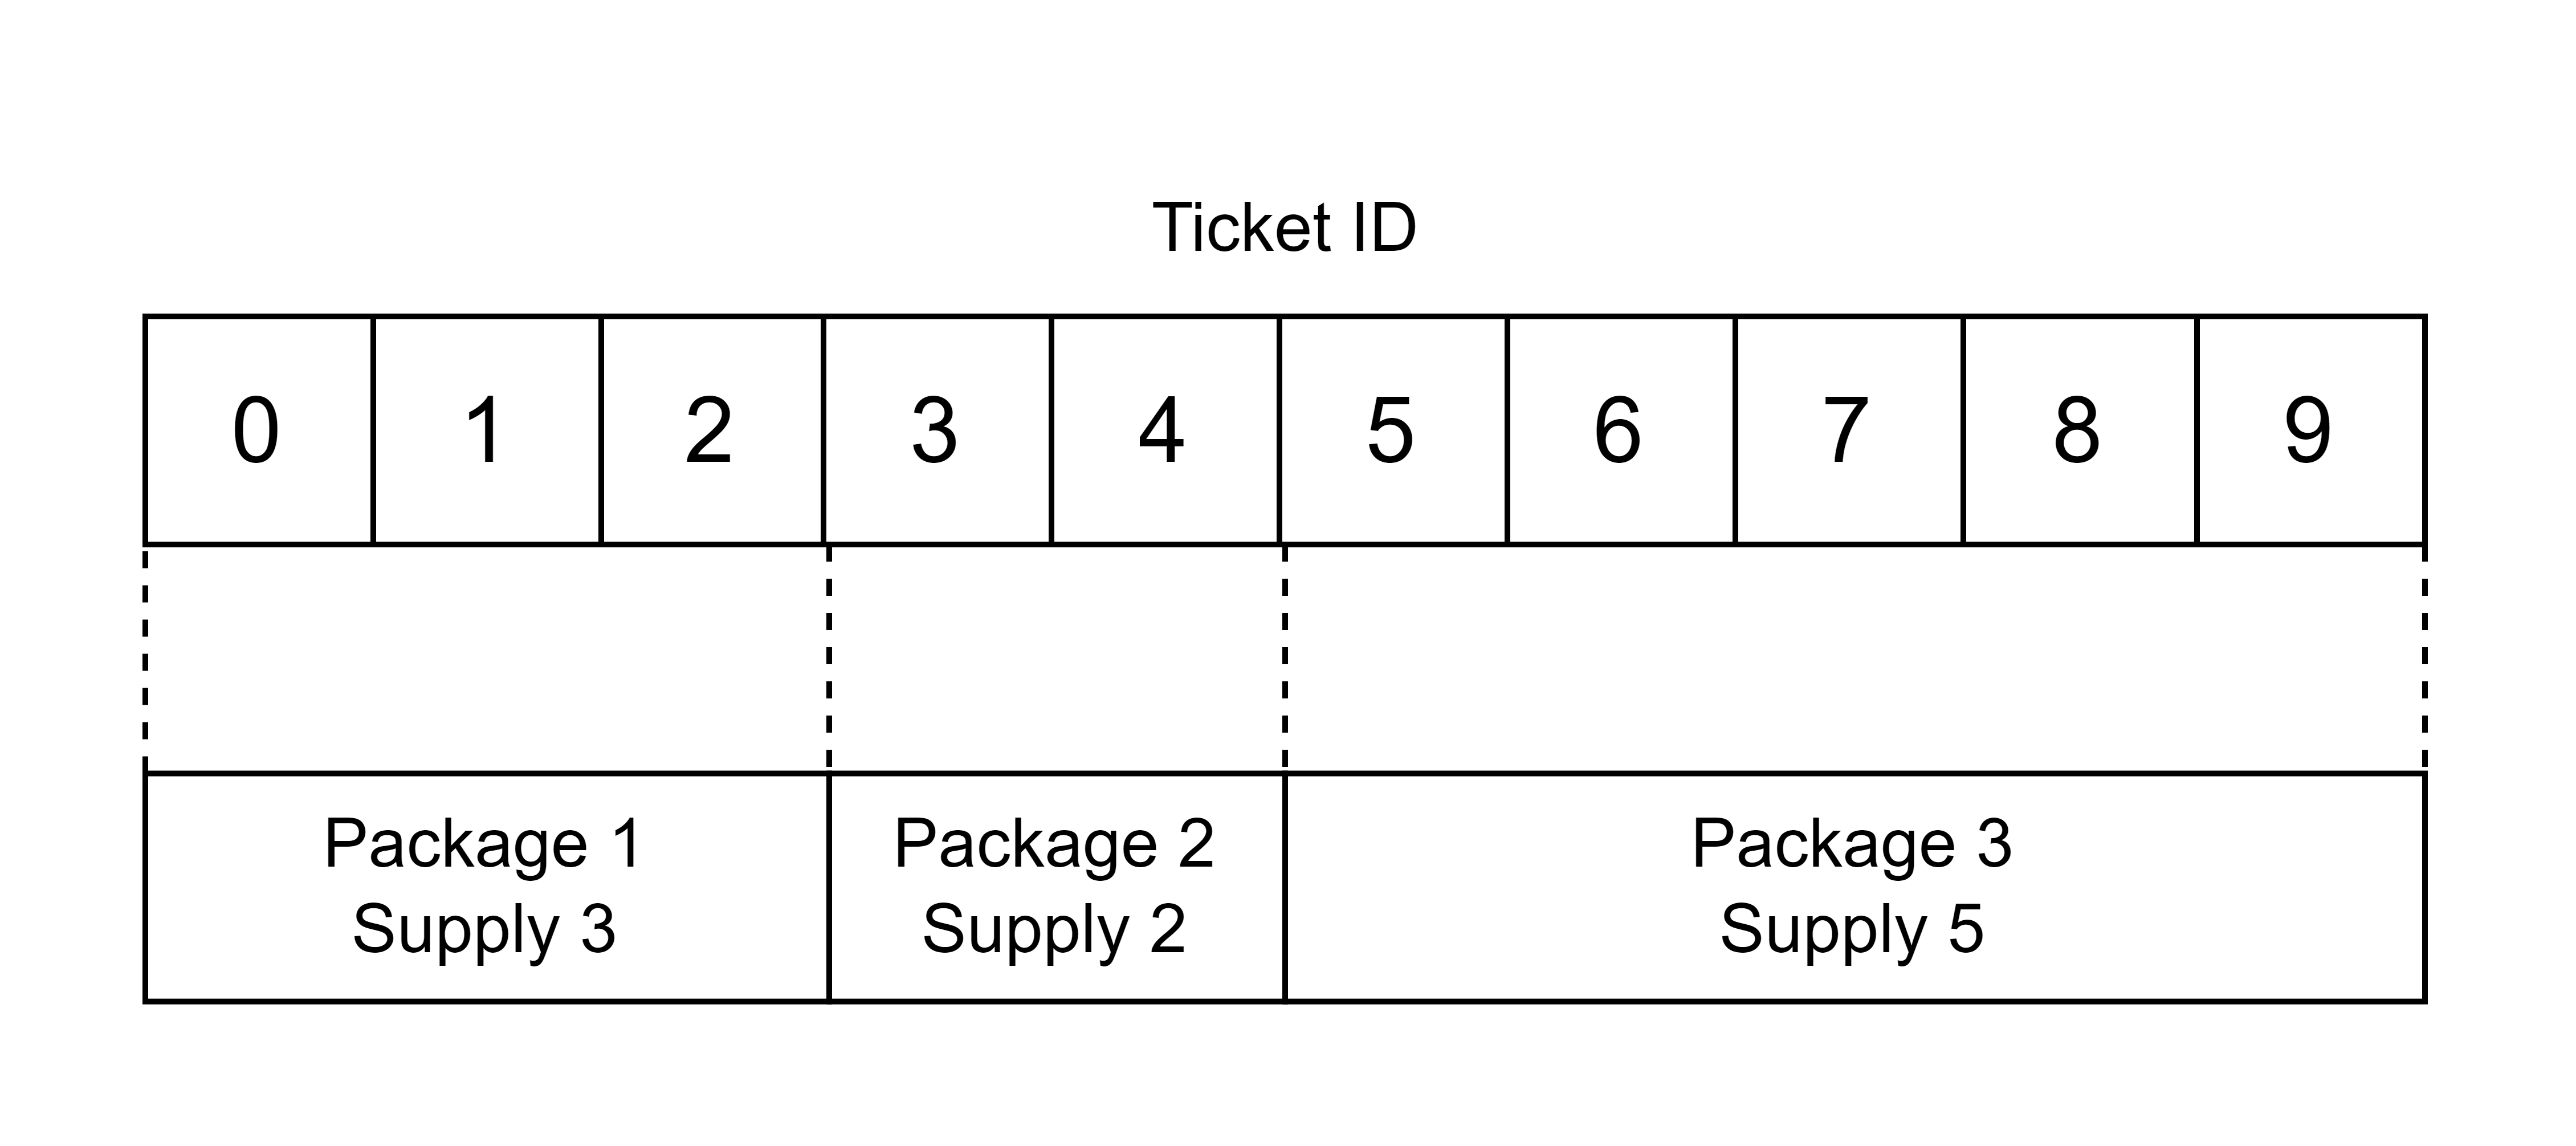
\includegraphics[width=\textwidth*2/3]{Package logic.png}
    \centering
    \caption{Package logic}
    \label{fig:package_logic}
\end{figure}

This way, whenever we need to get a ticket for a certain package, we can go through the packages and see in which one the ID is. One only limitation with this is if the event is already open (users can buy tickets), the only thing we can allow the organizer to do is to add packages, neither remove or change their order, because that would change the ID of the ticket, which would be a problem for the users that already bought them.

Now we just have to make sure the information obtained with the \textit{tokenURI} method corresponds to the ticket, according to its package. For this we will have a different metadata file for each package, with the necessary information about the tickets. The \textit{individualNfts} boolean in the \textit{PackageConfig} struct is there to indicate if the organizer wants each ticket on the package to have its own metadata, or if they can share it.

According to this, the \textit{tokenURI} will return an URI like 'baseURI/packageId/ticketId' for a package with individual NFTs, and 'baseURI/packageId' for a package with shared metadata. Like this, when we store the metadata on the IPFS, we store the metadata for each ticket inside a folder of the packages with individual NFTs, and only a metadata file for each package without individual NFTs.

\subsection{Metadata Storage}
\label{subsec:metadata_storage}

As we mentioned before, we'll be using the InterPlanetary File System (IPFS) for storing the NFTs metadata. The IPFS is a decentralized storage system where the data is stored in a distributed network of nodes (decentralized), making it very secure and reliable. This is a great solution for storing the metadata of the NFTs because it's very cheap and easy to use, and it's a common practice in the blockchain ecosystem. Other options would be to store the data on some kind of server, but that would be more expensive to maintain, and since we are dealing with NFTs, it's good practice to store the data in a decentralized manner, to avoid any kind of alteration on its contents, if the tickets possibly become valuable collectibles.

This kind of issue was something that has happened before, where people bought NFTs with the idea of them being somewhat valuable, but then the owner changed the contents of the metadata, executing what was called of a \textit{rug pull}, which is a scam that made the NFTs worthless, keeping the money for himself.

To store the data on the IPFS, we will be using the \href{https://www.pinata.cloud/}{Pinata} service, which does the heavy lifting for interacting with the storage itself. To accomplish this, we just need to arrange the files according to the ticket packages, like mentioned before in the Section \ref{subsec:ticket_packages}, and then upload them to the IPFS, getting the link to the metadata, which we'll then store on the contract as the base URI. The files would be stored like the Figure \ref{fig:metadata_storage} shows, being the packages 1 and 3 with shared metadata, and the package 2 with individual NFTs.

\begin{figure}[H]
    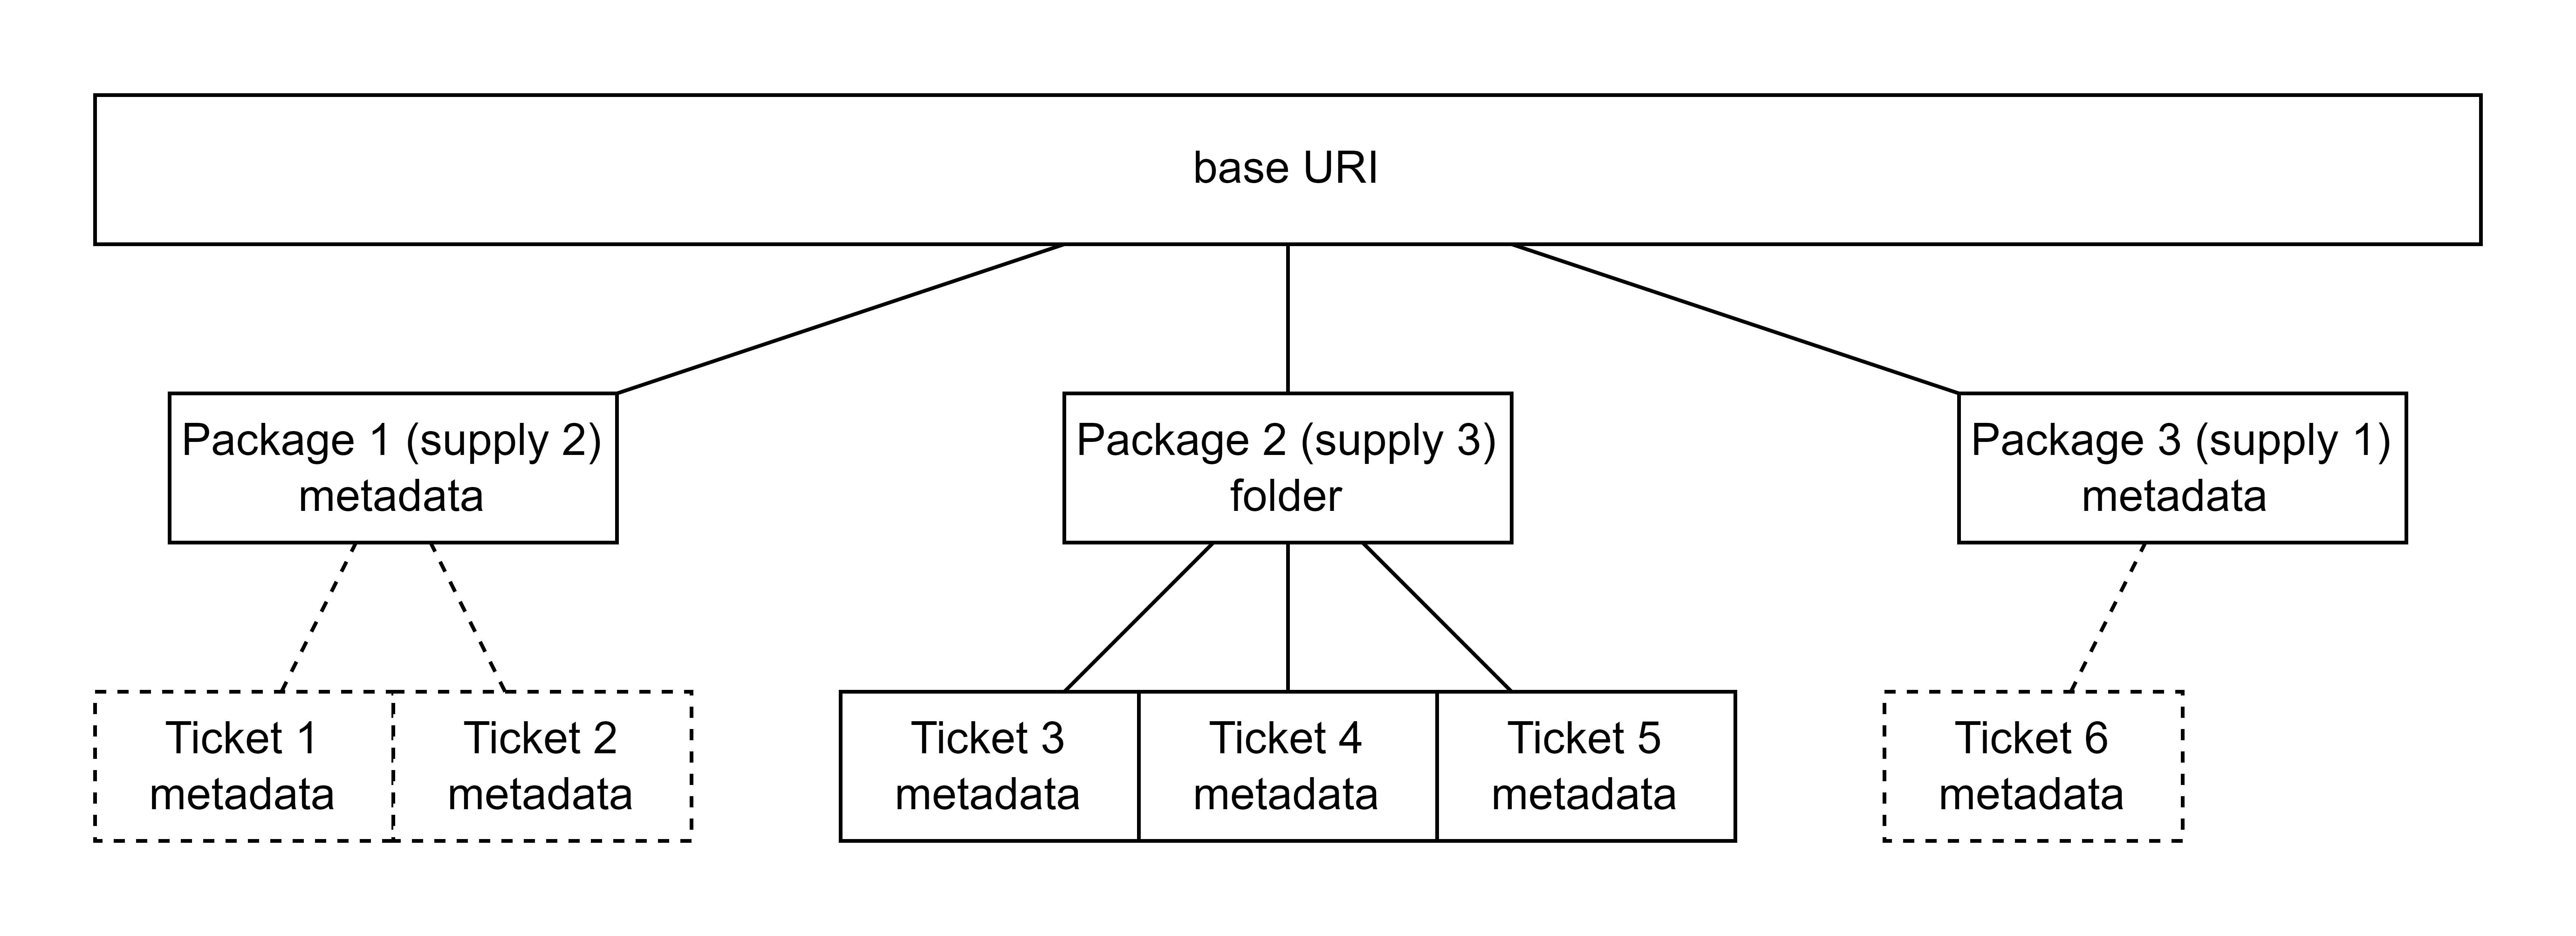
\includegraphics[width=\textwidth]{Metadata storage.png}
    \centering
    \caption{Metadata storage}
    \label{fig:metadata_storage}
\end{figure}

\subsection{System Fees}
\label{subsec:system_fees}

One of the most important aspects of a system like this is the business model we have to take into account. Since this is a service we want to deploy for event organizers, we need to make this sustainable and profitable. This kind of service aims to do some heavy lifting, with its own features, so we could set a fee lower than the usual on the traditional marketplaces and ticket selling platforms, since the organizers need to pay for each service.

These low fees are possible because with the system being deployed on the blockchain, it stays there while the network is running, so the only extra cost are the network fees when interacting with the event. For the users, each interaction is paid by them, so when a user buys a ticket, the only thing to take into account are the network fees, which depending on the network, can be super low.

The other kind of fee the organizer needs to look out for is for the validators to validate the tickets, which is a necessary operation to avoid people from exploiting the system. These fees are paid by the validators, which the organizer essentially manages, so we need to take this into account when setting the system fee, to make it sustainable for the organizer to use our system.

We'll set a fee on the main smart contract, where will be stored in the event when registering it, so that if we decide to change it, the previous events aren't affected. This is also because we want to abstract the user of any extra fee, so the price the organizer sets, is the price the user pays, and the system fee is taken from the tickets price. In case an event gets cancelled, or a user decides to get a refund, the ticket fee is returned to the user (proportional to the refund), making the system less profit, but guarantees the users of a fair process. With this, we need to restrict the system to only withdraw any profit after the event is over. Since this is rather an uncommon case, the less profit that the system makes compensates for the trust that the users and organizers will have on it.

\subsection{Ticket Validation}
\label{subsec:ticket_validation}

For the ticket validation, we must take into consideration a lot of aspects, because it's not just checking if the user address has a ticket associated to him. This is because, since the data is on the blockchain, anyone can see the addresses where each ticket belongs to, and pretend he's the owner of the ticket. For this to be secure, we need to guarantee the user is actually the owner of the address, and here is where the cryptographic message signature comes in, the same process that happens when executing a normal blockchain transaction.

Essentially the user will have to sign a message for the validator to check if the signature is valid, and if it is, it means the user is the actual owner of the ticket. There's a cryptographic method to recover the address of the signer using the original message and it's signature.

Knowing this, both parties need to know the original message so it matches. We could just use a default message for everyone, so the users would just need to give the signature to the validator, but this could become a security issue, in case the signature gets leaked, anyone who has it, could pretend to be a different address. The idea here is to have a unique message for each user at the time of the event, so it forces the user to sign it in the moment.

The process defined is shown in the Figure \ref{fig:ticket_validation}, where the user reads the QR with a generated message from the validator, signs it with his wallet, and generates a JSON with the signature and useful information like the tickets to validate, the event, and the user address. After the validator reads the JSON in the QR code, he checks if the parameters match the ones on the blockchain, gets the address from the signature and the message, and checks if the user is the owner of the tickets. If everything matches, the validator will trigger a transaction to mark the tickets as validated, to avoid people sharing the accounts and using the same ticket multiple times.

\begin{figure}[H]
    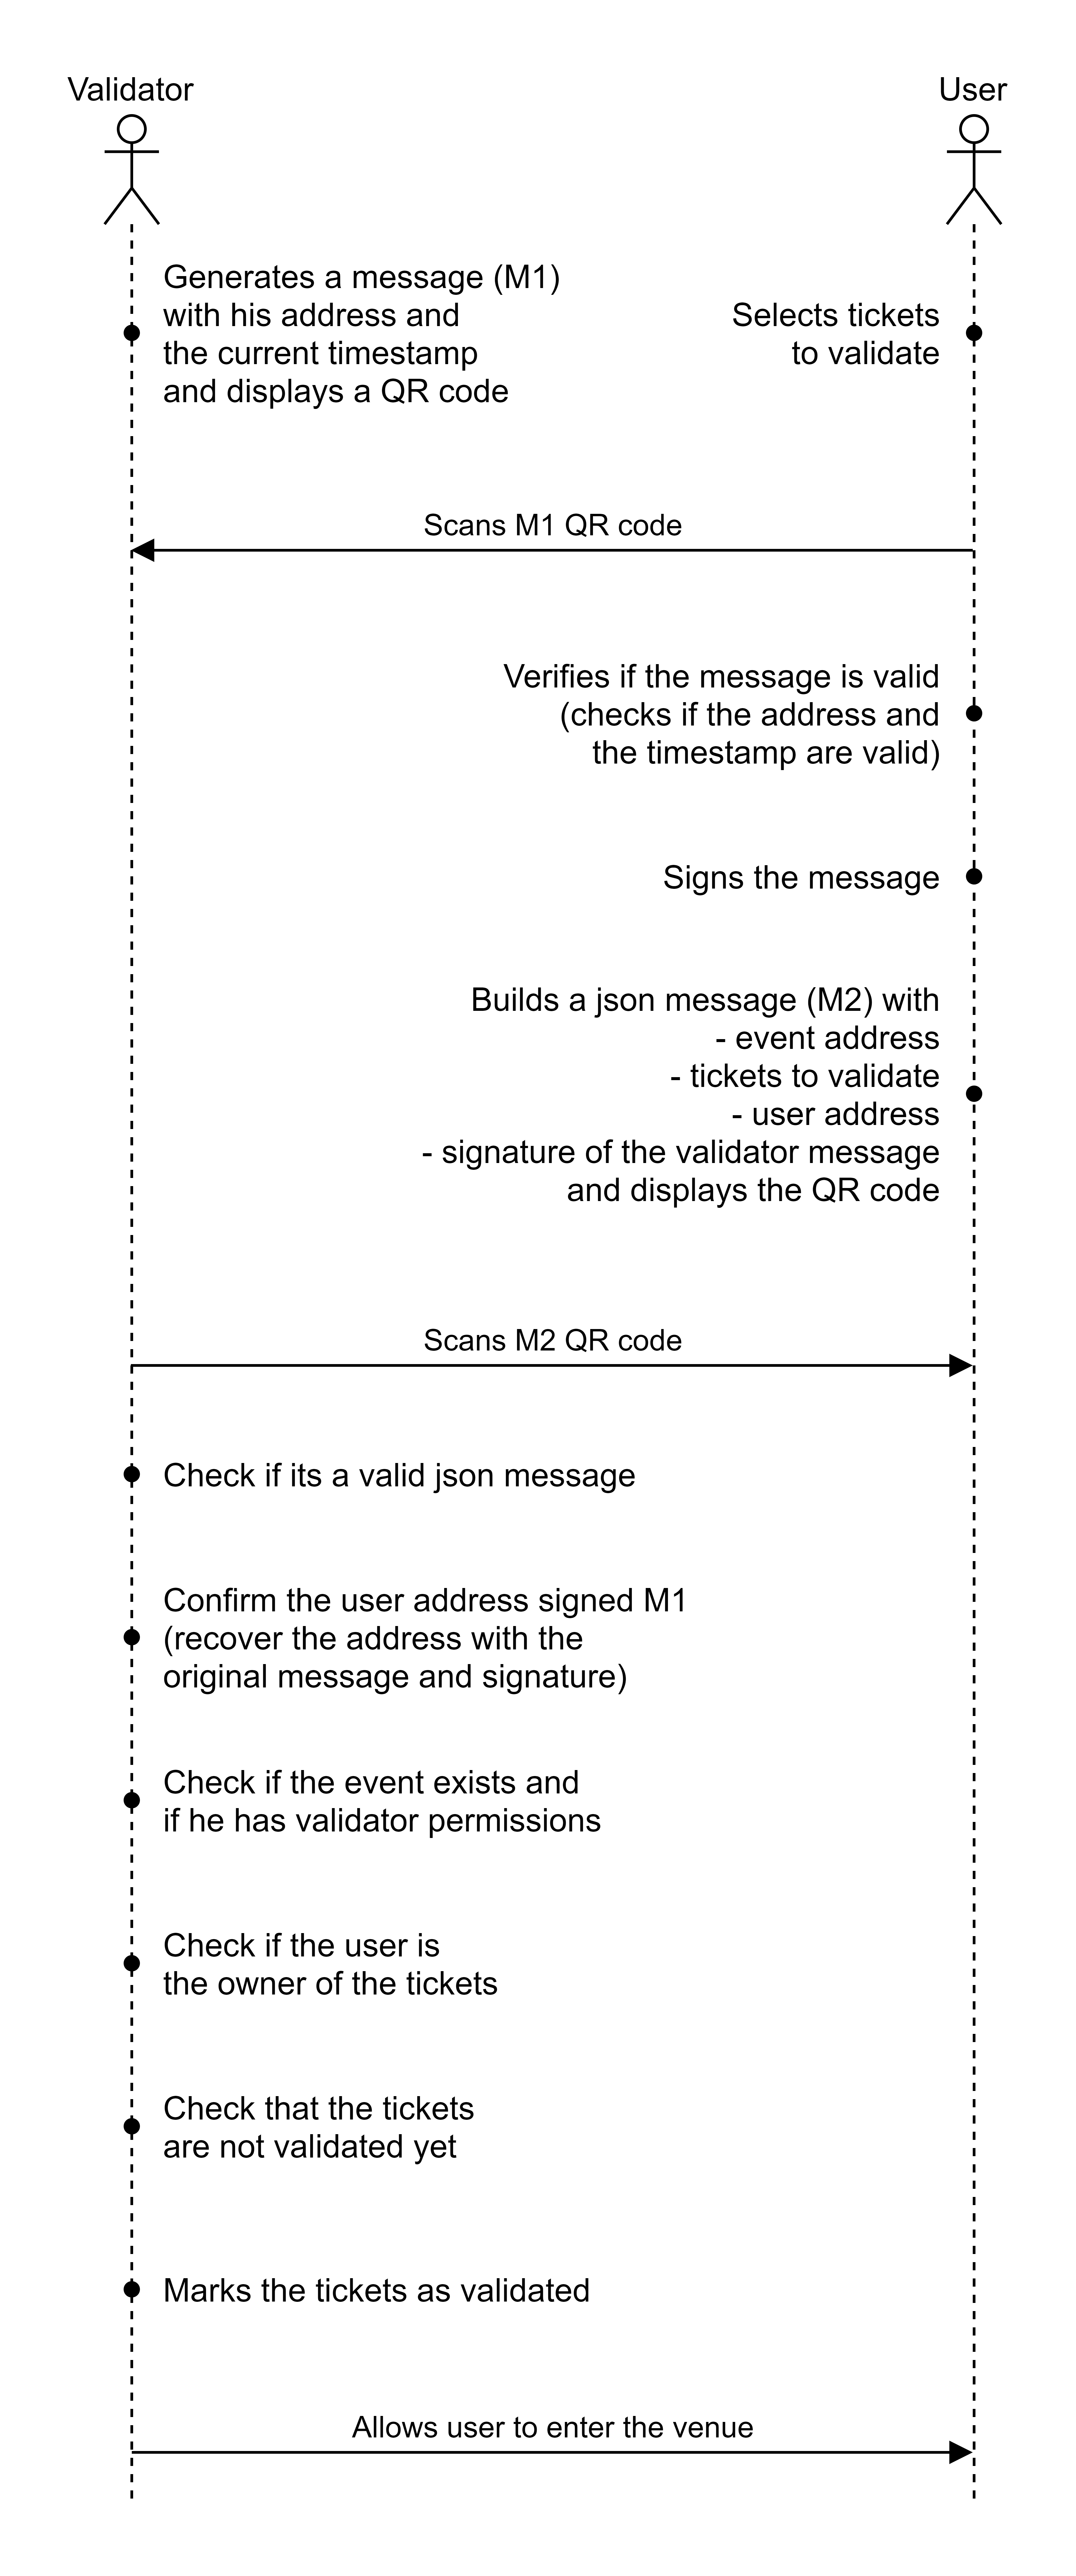
\includegraphics[width=\textwidth*3/5]{Ticket validation.png}
    \centering
    \caption{Ticket validation}
    \label{fig:ticket_validation}
\end{figure}

All this is reduced to a single transaction on the blockchain because, depending on the network, the finality of a transaction (the time it takes for a transaction to be fully registered on the blockchain) can take a while. This will be discussed in the next Section \ref{sec:network_choice}. This was planned to be done in a single transaction to avoid congestion at the entrance of the venue, so the users can enter the event with the least amount of delay.

\section{Network Choice}
\label{sec:network_choice}

The network choice is a very important aspect of the project, because it defines the limitations and the costs of the system. We want to aim for a blockchain that has low fees, is fast, secure and scalable, and since this is done using solidity, we have to aim for an EVM compatible network. To see which network matches our requirements, we need to analyze the statistics of the most popular EVM compatible networks, because these are the more secure ones.

Following the Figure \ref{fig:network_comparison}, we can see the main differences between the networks with the highest transactions per second (TPS). The main aspects to take into account from this figure are the TPS and the finality.

\begin{figure}[H]
    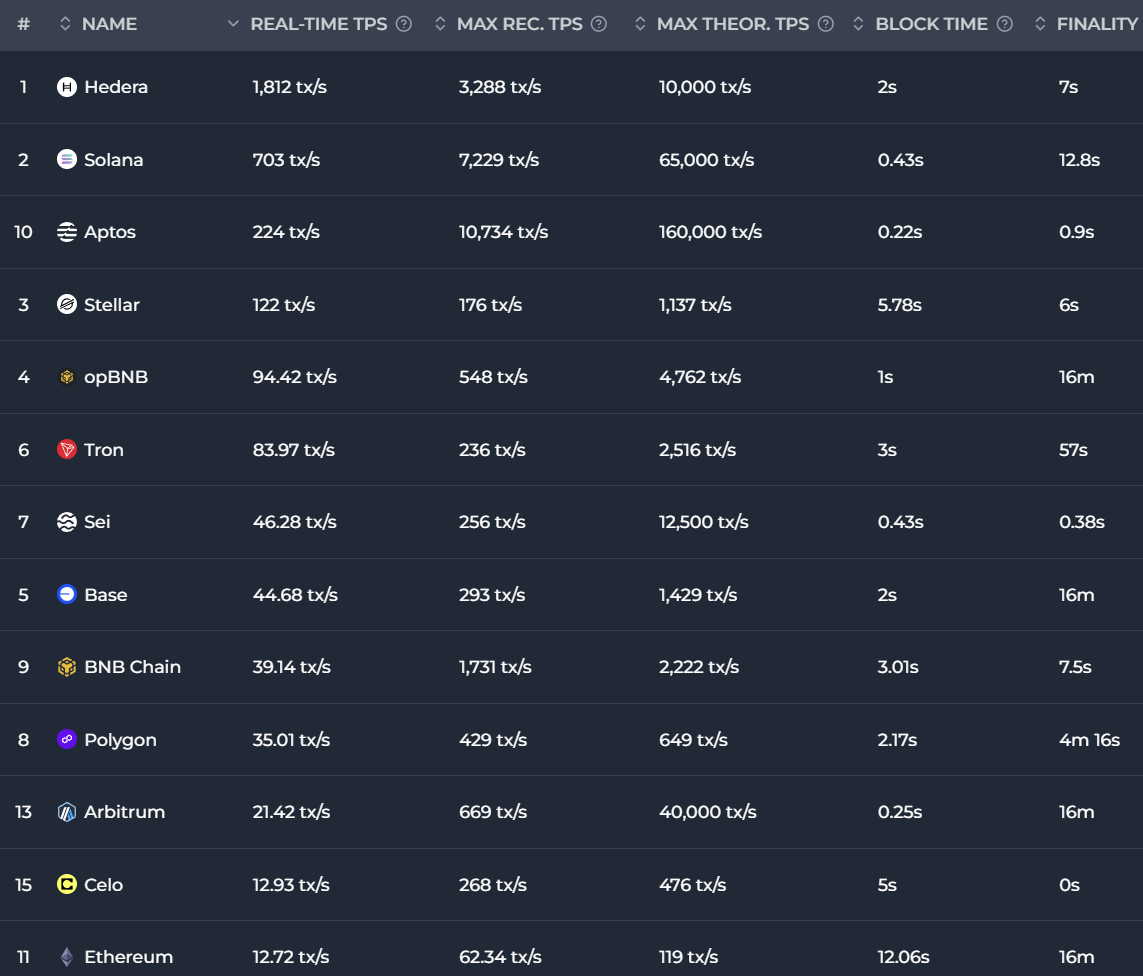
\includegraphics[width=\textwidth*2/3]{Network comparison 1.png}
    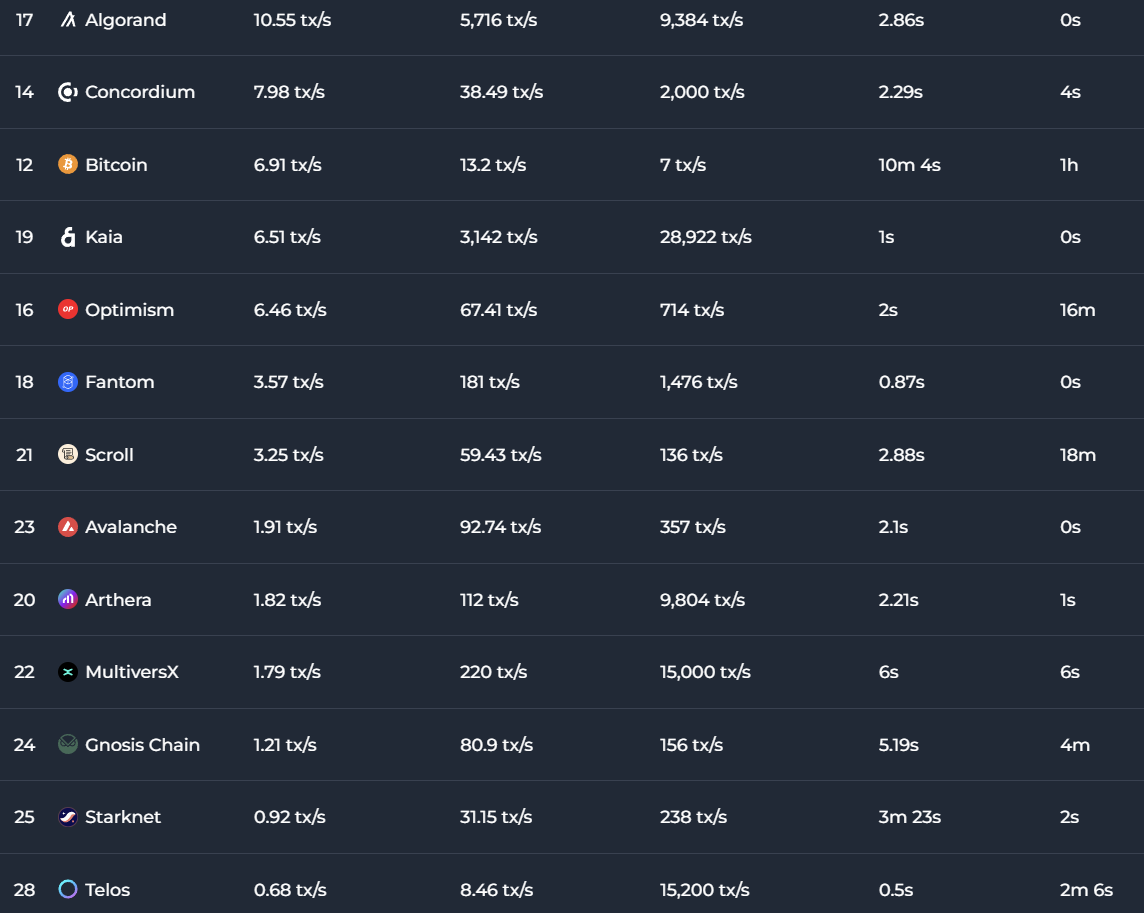
\includegraphics[width=\textwidth*2/3]{Network comparison 2.png}
    \centering
    \caption{Network comparison. Extracted from ...}
    \label{fig:network_comparison}
\end{figure}

Blockchains with higher TPS means they are more scalable, meaning they can process that amount of transactions in one second. Similar to how Visa and Mastercard work, they can process thousands of transactions per second, so the users don't have to wait for a long time for the transaction to be processed. In our case, a high TPS is important, but even more is the finality.

The finality is the time it takes for a transaction to be fully registered on the blockchain, meaning the time it takes for the transaction to be irreversible. This is important because we want the users to be able to enter the event as soon as possible, so the transaction to validate the tickets must be as fast as possible. This is the value that, if it takes too long, we will be waiting for each user individually to enter the event, which would be a problem. It's possible to see Ethereum down there, which has an average of 16 minutes for the finality, which is way too much for what we need.

Unfortunately a lot of networks there are not EVM compatible, so we have to choose between the ones that are. The two options that we could consider are the BNB Chain (also known as Binance Smart Chain (BSC)) and the Avalanche, being the first one the most popular and with higher scalability, but the second one has a way better finality.

The Avalanche chain would be the best bet, but having close to 2 tx/s (transactions per second), maybe its not scalable enough. For the BSC, it has a good enough finality and a good TPS so it would be a good choice for the project. This chain is also very popular and was created by Binance, one of the biggest companies in the blockchain ecosystem, so it's very secure and reliable.

\subsection{Fees}
\label{subsec:fees}

With this in mind, we still need to take into account the network fees. If this chain had high fees, then we would be forced to switch to another. Luckily, the BSC has very low fees, as the Figure \ref{fig:network_fees} shows, being the peak at 0.50 USD. Note that these are the fees to pay for a transaction, so if a user wants to buy multiple tickets, he can make it all at once instead of several individual purchases.

\begin{figure}[H]
    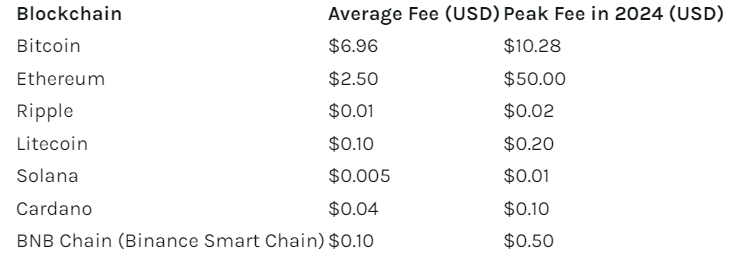
\includegraphics[width=\textwidth*2/3]{Network fees.png}
    \centering
    \caption{Network fees. Extracted from ...}
    \label{fig:network_fees}
\end{figure}

These fees are necessary as they are the cost for making the network run. This is common in the blockchain ecosystem, and it's a way to maintain the network secure and reliable, because the people processing the transactions are rewarded for their work, so they have an incentive to keep the network running. So we can never run away from this kinds of fees, but we can choose networks that have lower fees, so the users pay the least amount possible.

\section{User App}
\label{sec:user_app}

So the user app is a simple interface for the users to interact with the system, where they can authenticate, see the events, and buy and manage tickets. It will have a main page to check the events and a page for each event, where the user can see the details and buy the tickets, and will also have a page to see the tickets he owns.

For the authentication, we will use the service \href{https://walletconnect.com/}{Wallet Connect}, which supports a variety of wallets to interact with. What this service does is establish a connection between the app and a wallet, so that when a function needs to be called, the wallet receives the prompt and signs the transaction after the user's approval.

\section{Validator App}
\label{sec:validator_app}

For the validator app, we will have a simple interface for the validators to do the process mentioned in the Figure \ref{fig:ticket_validation}.

~

[check if i should mention exactly what i did here (to ease the process) or if i should mention what it should actually look like (a private key give by the organizer to input)]
%  The app itself will behave as a wallet in this case, to make things simple. 
% So basically the app will generate a private key and when the validator validates the tickets, the app will sign the message with the private key and send it to the blockchain. Since this is done by our system, when the validator has the app, the organizer will need to pass him some funds

Since the validators need to sign the message, the organizer just has to make sure the validators have enough funds to pay for the transaction.

\section{NOTES [to remove]}

 [should i mention marketplace and organizer dashboard?]

 [should i include the setters and getters in the UMLs?]
